\chapter{偏極陽子固体標的}
我々は、陽子の偏極生成手法として、光励起励起三重項電子スピンを用いた動的核偏極(Triplet-DNP)を用いている。
また、陽子偏極の偏極度測定方法として核磁気共鳴(NMR)を利用している。
本章では、まず陽子の偏極生成原理について説明し、その後NMRを利用した偏極の検出方法について述べる。

\section{偏極}
静磁場中の水素原子核スピン(I=1/2)は$|+1/2>, |-1/2>$いずれかのエネルギー固有状態となり、この各準位の占有数の偏りを偏極度という。
\begin{equation}
  P=\frac{N_+-N_-}{N_++N_-}
\end{equation}
一つのスピンの持つ磁化の大きさは
\begin{equation}
  \mu=\frac{1}{2}{\gamma_H} \hbar
\end{equation}
より、全体の磁化の大きさは
\begin{equation}
  M=N \mu P
\end{equation}
で表される。

\section{光励起励起三重項電子スピンを用いた動的核偏極(Triplet-DNP)の原理}
本研究では、偏極陽子標的としてナフタレンに重水素化ペンタセンを少量ドープした単結晶を用いている。
そして、ナフタレン内の水素原子核(陽子)の偏極生成手法として光励起励起三重項電子スピンを用いた動的核偏極(Triplet-DNP)を用いている。
この方法では、主に以下の3つの過程により陽子標的の偏極を行っている。

\begin{itemize}
  \item パルスレーザによる重水素化ペンタセン電子の偏極
  \item 電子スピンからナフタレン中の${}^1\rm{H}$スピンへの偏極移行
  \item 偏極拡散
\end{itemize}
本節では、この3つの過程に沿ってTriplet-DNPの基本原理について説明する。

\subsection{パルスレーザによる重水素化ペンタセン電子の偏極}
電子の偏極には、重水素化ペンタセンの光励起励起三重項電子スピン状態を利用している。
図$\ref{triplet_state}$に重水素化ペンタセンのエネルギー準位を示す。

\begin{figure}[tbp]
  \centering
  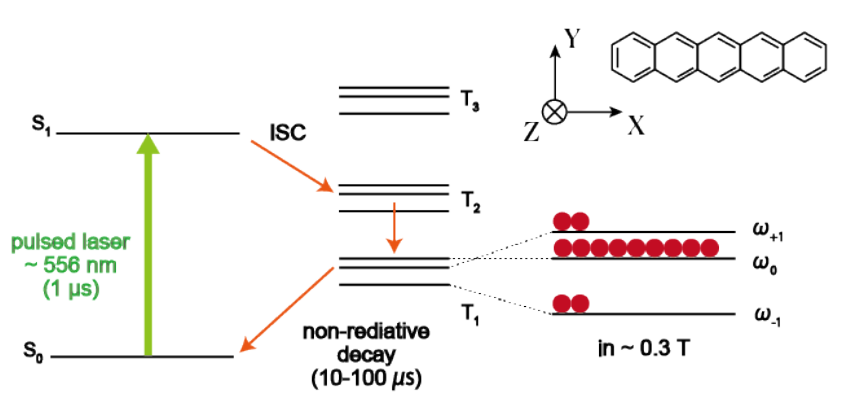
\includegraphics[clip,width=10cm]{./chap2/fig/triplet_state.png}\\
  \caption{重水素化ペンタセンのエネルギー準位図}
  \label{triplet_state}
\end{figure}

まず、600 nm以下の波長のパルスレーザの照射によって、基底状態($S_0$)から励起一重項状態($S_1$)へと重水素化ペンタセンの電子が励起される。
この$S_1$状態の電子は寿命$\sim 20$ nsで大半は基底状態($S_0$)に脱励起するが、わずかに$T_2$状態を経由して、最低次のスピン三重項状態である$T_1$状態に無放射的に脱励起するものが存在する。

このように、スピン多重度が異なる状態間の無放射遷移は項間交差(intersystem crossing)と呼ばれる。
これは禁制遷移だが、スピン軌道相互作用に起因する状態間の混合により生じる。\\
項間交差の選択性により、遷移する際に三重項状態の各準位間に占有数の差が生じる。
この占有数の差が電子の偏極である。

% 河原修論P6%
また、この占有数の差は外部磁場の方向と、重水素化ペンタセン分子の分子軸の間の角度によって変化する。
ここでペンタセン分子の分子軸と外磁場の向きを図$\ref{pentacene_axes}$に示すように定義すると、


\begin{figure}[ht]
  \centering
  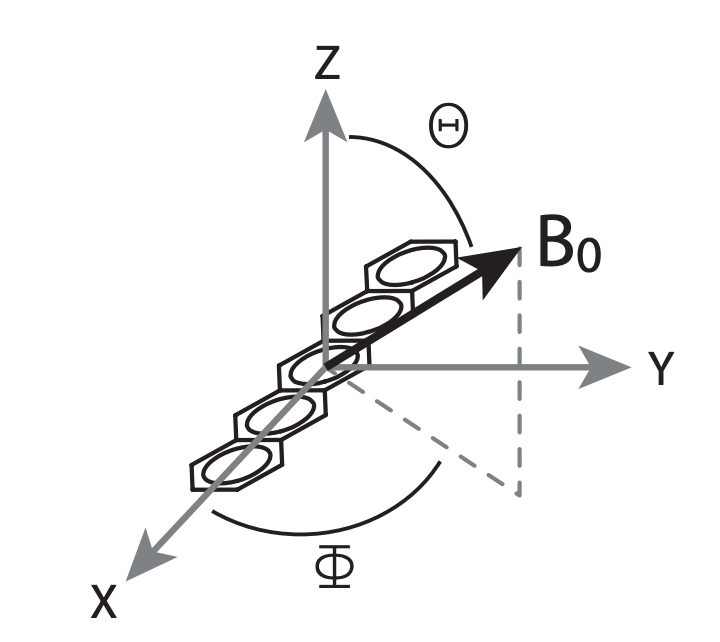
\includegraphics[keepaspectratio, scale=0.5]
       {./chap2/fig/pentacene_axes.png}
  \caption{ペンタセン中のZFSテンソルの主軸系}
  \label{pentacene_axes}
 \end{figure}

 \begin{figure}[ht]
  \centering
  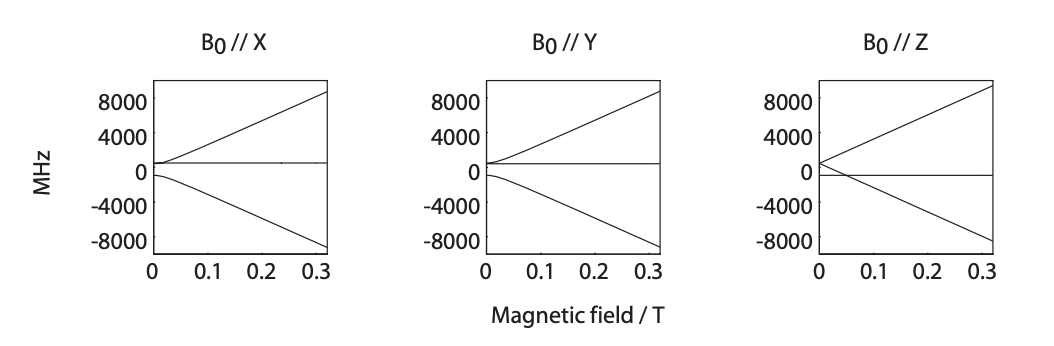
\includegraphics[keepaspectratio, scale=0.5]
       {./chap2/fig/energysplit_B0.png}
  \caption{ペンタセン分子軸と三重項副順位間の占有数の差$\cite{David}$}
  \label{energysplit}
 \end{figure}

 図$\ref{energysplit}$より、ペンタセン分子の長軸と外磁場が平衡であるときに各準位間の電子の占有数の差が
 最大になることがわかる。
 この時の三重項状態での占有数の割合はN(+1):N(0):N(-1)=12\%:76\%;12\%である$\cite{David}$。
偏極生成過程で用いるのは3つの副準位の占有数の差であるので、この2つの副準位だけを考える。この時、占有数の偏りの最大値は以下のように表される。
\begin{equation}
  \it P_{max}=\frac{\rm{N}(0)-\rm{N}(-1)}{\rm{N}(0)+\rm{N}(-1)}=\frac{\rm{76}(\%)-\rm{12}(\%)}{\rm{76}(\%)+\rm{12}(\%)}=\rm{73}(\%)
  \label{pentacene_P}
\end{equation}
この偏りは外磁場の方向とペンタセンの分子軸との間の角度だけに依存しており、外磁場の強さや温度には囚われないため高温、低磁場中でも$73\%$の電子偏極($P_e$)を得ることができる$\cite{David}$。
そして最後にこの$T_1$状態の電子は基底状態$S_0$に脱励起する。$T_1$状態では副順位間で寿命も異なる。
温度100 Kで報告されている値は$m_s=0$の時には$26 \mu sec$で、$m_s=\pm 1$の時には$83 \mu sec$である$\cite{Iinuma}$。

%丸田修論p20%
通常のペンタセンでも偏極は可能であるが、本研究では重水素化されたペンタセンを用
いている。これはペンタセンの代わりに重水素化ペンタセンを
ナフタレンにドープすることで、偏極度が向上することが確認されているからであ
る$\cite{Tateishi}$。ペンタセン中の ${}^1\rm{H}$ スピンは電子スピンが非常に近くに位置しているので、電子
スピンと強く結合し、電子${}^1\rm{H}$ 偏極交換の担い手になっている。しかし、同時に電子から
非常に強い緩和を受けているため、${}^1\rm{H}$ スピンの緩和時間を押し下げている。そこで、重
水素化ペンタセンを用いることでこの緩和を抑制し、偏極度を向上させることができる。
なおこれにより偏極交換は、遠くにある(結合強度の小さい)ナフタレン中の ${}^1\rm{H}$ ス
ピンと行わなければならなくなるが、ICP パラメータの調整次第で、通常のペンタセンと
ほぼ同等の効率で偏極交換ができる。

\subsection{電子スピンから${}^1\rm{H}$スピンへの偏極移行}
電子スピンと ${}^1\rm{H}$ スピン間の偏極交換には、Integrated Corss Polarization 法 (ICP)
と呼ばれる方法を用いる。この方法では、以下の式$\ref{Hartmann-Hahn}$を満たすとき、電子スピンの高
偏極状態が  ${}^1\rm{H}$スピンへと移行される。

\begin{equation}
  \omega_{eff e}=\omega_{0 H}
  \label{Hartmann-Hahn}
\end{equation}

ここで$\omega_0 H$は${}^1\rm{H}$スピンのラーモア周波数、$\omega_{eff e}=\sqrt{\omega^2_{1e}+\Delta\omega^2_e}$は電子スピンの実効磁場強度で、$\omega_{1e}$は電子スピンのラビ周波数、$\Delta\omega_e$はオフセット周波数である。
つまり、電子スピンの実効的なラビ周波数と ${}^1\rm{H}$ スピンのラーモア周波数を一致させるこ
とが偏極移行のための条件であり、式 $\ref{Hartmann-Hahn}$ は Hartmann-Hahn 条件と呼ばれる。この
Hartmann-Hahn 条件を満たした時、電子スピンと ${}^1\rm{H}$ スピンの超微細結合ハミルトニア
ンがフリップフロップ項を持ち、電子スピンの偏極が ${}^1\rm{H}$ スピンへ移行
される。しかし、電子スピンの共鳴周波数は、核スピンとの超微細結合によって不均一に
広がっている(図$\ref{spin_packet}$)。そのため、個々のスピンパケットが感じる実行磁場はそれぞれ異
なり、マイクロ波を電子スピンに照射しても一部の電子しか Hartmann-Hahn 条件を満
たすことができない。この問題は、Henstra の静磁場を掃引するというアイディアにより
解決された$\cite{Henstra1}$。

\begin{figure}[ht]
  \centering
  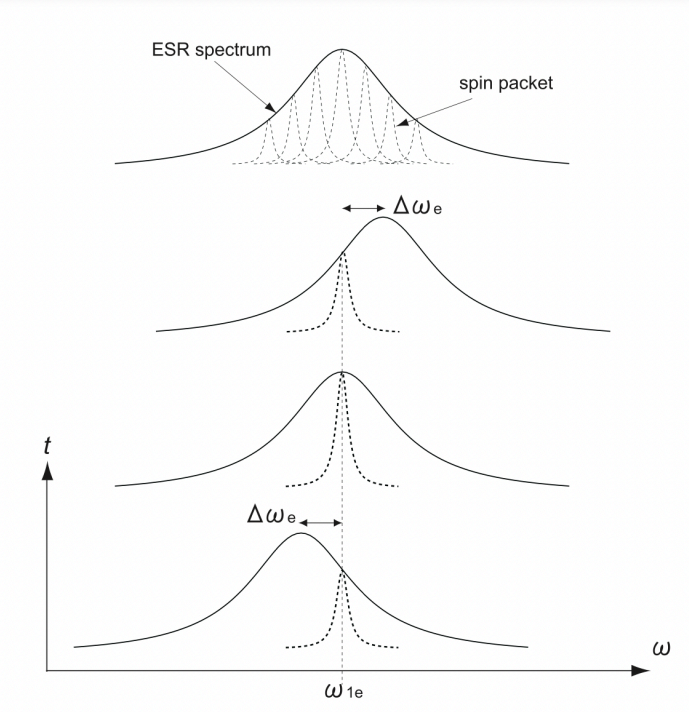
\includegraphics[keepaspectratio, scale=0.5]
       {./chap2/fig/spin_packet.png}
  \caption{電子スピンパケットの拡がりと電子スピン共鳴の磁場掃引}
  \label{spin_packet}
 \end{figure}

 この方法では、図$\ref{spin_packet}$のように、電子スピンの共鳴周波数が、
 照射するマイクロ波周波数よりも低くなる磁場から高くなる磁場まで掃引する。Henstra らはこの
 方法を Integrated Solid Effect(ISE) と名付けた$\cite{Henstra2}$。磁場掃引を含めた ICP のシー
 クエンスを図$\ref{pulse_sequence}$に示す。

 \begin{figure}[ht]
  \centering
  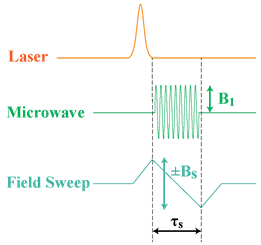
\includegraphics[keepaspectratio, scale=1.5]
       {./chap2/fig/pulse_sequence.png}
  \caption{ICPシークエンス}
  \label{pulse_sequence}
 \end{figure}

 磁場掃引を中心磁場 $B_0$、掃引幅 $B_S$ で、$\tau_S$ の間行う場合、磁場の時間変化 $B_0(t)$ は以
 下の式$\ref{B0t}$のように書ける。

\begin{equation}
  B_0(t)= B_0 \pm \frac{B_S}{\tau_S}(t-\frac{\tau_S}{2})
  \label{B0t}
\end{equation} 

磁場の掃引が以下の式$\ref{Insulation conditions}$で表される断熱条件を満たすときに、電子スピンパケットは
実効磁場の方向にロックされていく [44]。

\begin{equation}
  \gamma_e\frac{dB_0(t)}{dt} \ll \frac{\omega^2_e}{\rm{sin}\alpha(t)}
  \label{Insulation conditions}
\end{equation}

ここで$\alpha (t)$は、静磁場と実効磁場のなす角である。磁場の掃引方向を変えることで、正
偏極生成と負偏極生成を変えることができる。

\subsection{スピン拡散}
${}^1H$ スピンが数多く存在している系の回転座標系のハミルトニアンは、以下の式$\ref{Hamiltonian}$のように書ける。

\begin{equation}
  \mathcal{H}_{II}={\displaystyle \Sigma_{j,k}}d_{j,k}[2I_{jz}I_{kz}-\frac{1}{2}(I_{j+}I_{k-}+I_{j-}I_{k+})]
  \label{Hamiltonian}
\end{equation}

$I_j$ は j 番目の I スピンのスピン演算子で、$d_{j,k}$ は j 番目と k 番目の I スピン間の双極子
相互作用の結合定数である。$d_{j,k}(I_j+I_k− + I_{j−}I_{k+})/2$ はフリップフロップ項であり、お
互いのスピンの z 成分を交換させる働きがある。全ての I スピン間で偏
極率の交換が行われているため、物質中で偏極率に空間的偏りがある場合には、この交換
によってその空間的偏りはならされていく。この熱拡散のような現象はスピン拡散と呼ば
れている。

\subsection{Triplet-DNPによる偏極の蓄積}
ICP 後、三重項状態は無放射遷移で、元の基底一重項状態 $S_0$ へと戻る。重水素化ペン
タセン近傍に局在する ${}^1H$ スピンの高偏極状態はスピン拡散により周囲のホスト分子の
${}^1H$ スピンへ移っていく。ペンタセン近傍の高偏極状態が標的サンプル全体に拡散した後、
再びパルスレーザによる光励起、マイクロ波照射による ICP を行えば、さらに高偏極状
態を積み重ねることができる。この過程を何度も繰り返していくことで、${}^1H$ スピンに高
偏極状態を蓄積することができる。
飯沼・武田らは、Triplet-DNP による ${}^1H$ スピン偏極率 P の上昇の様子を、偏極生成
時定数 ${T_D}$ とレーザ照射時の偏極緩和時定数 $T_{1laser}$ を用いて、以下の式のような
レート方程式で表現できることを示した$\cite{Takeda}$。

\begin{equation}
  \frac{dP}{dt}=\frac{1}{T_D}(P_e-P)-\frac{1}{T_{1laser}}(P-P_{th})
  \label{pol_dif}
\end{equation}
ここで、$P_e$ は電子スピンの偏極率、$P_{th}$ は ${}^1H$ スピンの熱平衡状態の偏極率である。ま
た、$T_{1laser}$ は ${}^1H$ スピンのスピン-格子緩和時間 $T_1$ と、${}^1H$ スピンとの偏極交換に使われ
なかった残留偏極電子による緩和 $T_e$ を用いて以下の式$\ref{T_{1laser}}$のように表せる。

\begin{equation}
  \frac{1}{T_{1laser}}=\frac{1}{T_1}+\frac{1}{T_e}
  \label{T_{1laser}}
\end{equation}

本実験条件では $P_{th}$ は非常に小さいため、$P_{th}$ を無視して式を解くと以下の解$\ref{pol}$を得る。

\begin{equation}
  P(t)=\frac{P_e}{1+\frac{T_D}{T_{1laser}}}\left[1-exp\left(-\left(\frac{1}{T_D}+\frac{1}{T_{1laser}}\right)\right)t\right]
  \label{pol}
\end{equation}


\section{陽子の偏極信号の検出}
陽子の偏極信号の検出には、NMR 法を利用する。

\subsection{NMRの基本原理}
\subsubsection{ゼーマン相互作用}
スピンIはZ軸方向にかけられた静磁場$\textbf{B}_0 = (0, 0, B_0)$ 中で、式$\ref{Zeeman}$のゼーマン相
互作用によってエネルギー分裂が生じる。

\begin{equation}
  \mathcal{H}_{Zeeman}=-\gamma B_0 I_Z=\omega_{0I}I_Z
  \label{Zeeman}
\end{equation}


ここで、$\gamma$ は磁気回転比、$\omega_{0I}$ はラーモア周波数である。またスピン演算子 $\textbf{I} = (I_x , I_y , I_z)$
は、パウリ行列:

\begin{equation}
  \textbf{1}=
  \begin{pmatrix}
    1 & 0 \\
    0 & 1 \\
  \end{pmatrix}
  ,
  \sigma_x=
  \begin{pmatrix}
    0 & 1 \\
    1 & 0 \\
  \end{pmatrix}
  ,
  \sigma_y=
  \begin{pmatrix}
    0 & -i \\
    i & 0 \\
  \end{pmatrix}
  ,
  \sigma_z=
  \begin{pmatrix}
    1 & 0 \\
    0 & -1 \\
  \end{pmatrix}
  \label{pauli_matrix}
\end{equation}
を用いて式$\ref{spin_operator}$で表される。
\begin{equation}
  I_x=\frac{\sigma_x}{2},
  I_y=\frac{\sigma_y}{2},
  I_z=\frac{\sigma_z}{2}
  \label{spin_operator}
\end{equation}
さらに、スピン昇降演算子$I_+,I_-$を以下の式$\ref{spin_updown}$で定義する。
\begin{equation}
  I_+=I_x+iI_y=
  \begin{pmatrix}
    0 & 1 \\
    0 & 0 \\
  \end{pmatrix}
  ,I_-=I_x-iI_y=
  \begin{pmatrix}
    0 & 0 \\
    1 & 0 \\
  \end{pmatrix}
\label{spin_updown}
\end{equation}

\subsubsection{密度演算子と回転座標系}
現実的な多粒子状態を考える場合、全ての粒子状態について一つ一つ記述することは不
可能である。そこで、以下の式で定義される密度演算子を導入する。
\begin{align}
\begin{aligned}
  \hat{\rho} &= \mathbb{N}^{-1}(\ket{\psi_1}\bra{\psi_1}+\ket{\psi_2}\bra{\psi_2}+\dots)\\
            &= \overline{\ket{\psi} \bra{\psi}}
\end{aligned}
\end{align}
スピン状態の密度演算子 $\rho$ の時間発展は、リウビル-フォンノイマン方程式$\ref{Liouville}$で記述できる。

\begin{equation}
  \frac{d}{dt}\rho(t)=i[\rho(t),\mathcal{H}]
  \label{Liouville}
\end{equation}
ハミルトニアンが時間依存しない時は、以下の式$\ref{Liouville2}$で状態の時間発展が記述できる。

\begin{align}
  \begin{aligned}
    \rho(t)&=&U\rho(0)U^{-1}\\
          U&=&\rm{exp}(-i\mathcal{H}t)
    \label{Liouville2}
  \end{aligned}
\end{align}

NMR によるスピンダイナミクスを理解しやすくするために、Z 軸まわりに $\omega I$ で回転
する回転座標系を導入する。回転座標系から見たスピン状態 $\rho^R$は、以下の式$\ref{rhoR}$で与えられる。

\begin{align}
  \begin{aligned}
  \rho^R(t)&=U(t)^{-1}\rho(t)U(t)\\
  U(t)&=\rm{exp}(-i\omega_I I_Z t)
  \label{rhoR}
  \end{aligned}
\end{align}
したがって、回転座標系のハミルトニアンは式$\ref{Hamiltonian_R}$のように与えられる。

\begin{equation}
  \mathcal{H}^R = U(t)^{-1}\mathcal{H}^R U(t)-iU(t)^{-1}\frac{d}{dt}U(t)
  \label{Hamiltonian_R}
\end{equation}

\subsubsection{双極子相互作用}
2 スピン($\textbf{I}$スピン、$\textbf{S}$スピン)間には双極子相互作用が働く。実験室座標系における
双極子相互作用のハミルトニアンは、以下の式$\ref{dipole_H}$で与えられる。

\begin{align}
  \begin{aligned}
    \mathcal{H}_{IS}&=b_{IS}\left[\frac{3(\textbf{I}\cdot \textbf{r}_{IS})(\textbf{S}\cdot \textbf{r}_{IS})}{r^2_{IS}}-\textbf{I}\cdot \textbf{S} \right]\\
    b_{IS}&=-\frac{\mu_0}{4\pi}\frac{\gamma_I \gamma_S \hbar}{r^3_{IS}}
    \label{dipole_H}
  \end{aligned}
\end{align}

ここで、$r_{IS}$ は核間ベクトル、$r_{IS}$ は核間ベクトルの長さ、$\mu_0$ は真空の透磁率、$\gamma_I\gamma_S$ は
$\textbf{I},\textbf{S}$ スピンの磁気回転比を表す。式$\ref{dipole_H}$の双極子相互作用ハミルトニアンは、以下の
式$\ref{dipole_H2}$で書き直すことができる$\cite{Abragam}$。


\begin{align}
  \begin{aligned}
    \mathcal{H}_{IS}&=b_{IS}(A+B+C+D+E+F)\\
    A&=(3cos^2\theta_{IS}-1)I_ZS_Z\\
    B&=-\frac{1}{4}(3cos^2\theta_{IS}-1)(I_+S_-+I_-S_+)\\
    C&=\frac{3}{2}sin\theta_{IS}cos\theta_{IS}e^{-i\phi}(I_+S_Z+I_ZS_+)\\
    D&=\frac{3}{2}sin\theta_{IS}cos\theta_{IS}e^{-i\phi}(I_-S_Z+I_ZS_-)\\
    E&=\frac{3}{4}sin^2\theta_{IS}e^{-2i\phi}I_+S_+\\
    F&=\frac{3}{4}sin^2\theta_{IS}e^{2i\phi}I_-S_-\\
    \label{dipole_H2}
  \end{aligned}
\end{align}
ここで $\theta_{IS}$ は Z 軸と核間ベクトルのなす角度である。静磁場下では、系のハミルトニア
ンは以下の式$\ref{H_Z}$のように書ける。

\begin{equation}
  \mathcal{H}=\omega_{0I}I_Z+\omega_{0S}S_Z
  \label{H_Z}
\end{equation}

ここで $\omega_{0I} , \omega_{0S}$ はそれぞれ I スピンと S スピンのラーモア周波数である。I スピンが
$\omega_{0I}$ で、S スピンが $\omega_{0S}$ でそれぞれ回転する座標系、すなわち二重回転座標系における系
のハミルトニアンは、以下の式 (B.13) で与えられる。

\begin{equation}
  siki
\end{equation}

$|\omega_{0I}-\omega_{0S}|\gg b_{IS}$  場合、すなわち異種核間の場合、$\omega_{0I} I_Z + \omega_{0S}S_Z$ は式$\ref{dipole_H2}$で示
される A とは可換で、その他の項とは非可換となる。この非可換な項の時間発展は平均
化され、ほとんど状態発展に寄与しないと考えて良い。よって、異核間双極子相互作用は
以下の式$\ref{H_DR}$のようになる。

\begin{equation}
  siki
  \label{H_DR}
\end{equation}

これをセキュラー近似(secular approximation)と呼ぶ$\cite{Levitt}$。
$\omega_{0I}=\omega_{0S}$場合、すなわち同核間の場合、$ \omega_{0I}(I_Z + S_Z) $は式$\ref{dipole_H2}$で示される A, B
とは可換で、その他の項とは非可換となる。よって、同核間双極子相互作用は、以下の式$\ref{H_DR2}$で与えられる。

\begin{equation}
  \label{H_DR2}
\end{equation}

式$\ref{H_DR2}$の$\frac{1}{2}(I_+S_− + I_−S_+)$ はフリップフロップ項と呼ばれている。初期状態$P_I I_Z +P_SS_Z +\frac{1}{4}$ の 2 スピン系にこのフリップフロップ項を$ \frac{\pi}{d_{IS}}$
秒間作用させると、以下の式$\ref{UFF1}$のように、I スピンと S の Z 成分を交換する。
\begin{equation}
  siki
  \label{UFF1}
\end{equation}
\begin{equation}
  siki
  \label{UFF2}
\end{equation}
すなわち、フリップフロップ項を作用させることは、偏極率を交換することに対応する。

\subsubsection{RF照射と自己誘導減衰}
Z軸方向の静磁場$B_0$下で、X軸方向のラジオ波(RF)磁場$B_{1I}(t)= - \frac{2\omega_{1I}}{\gamma_I}cos(\omega_It+\phi_I)$
照射下での、実験室座標系における I スピンのハミルトニアンは、以下の式$\ref{RF_H}$で与えられる。

\begin{equation}
  siki
  \label{RF_H}
\end{equation}

$\omega_I$はRF照射のキャリア周波数、$\phi_I$は初期位相である。$\omega_{1I}$はラビ周波数である。式
$\ref{RF_H}$で示したハミルトニアンを回転座標系において書き直すと、以下の式$\ref{RF_H2}$のようになる。

\begin{equation}
  siki
  \label{RF_H2}
\end{equation}

この時、回転波近似を用いた。
$\omega_{0I} = \omega_I$ のオンレゾナンス照射の場合、照射位相$\phi_I=0^\circ$で X 軸回りの$\theta$回転となる。

\begin{equation}
  siki
  \label{RX}
\end{equation}

RF 照射により得られる NMR 信号は量子力学的には、$I_-$ 演算子の期待値で表される。
\begin{equation}
  Tr[\rho I_-]
  \label{Tr}
\end{equation}
1 スピン系の場合、初期状態 $\rho_0 =\frac{1}{2}+P_{thI}I_z$ のスピンに $\frac{\pi}{2}$ パルスを作用させると、
以下の式$\ref{rho_2}$のようになる。

\begin{equation}
  siki
  \label{rho_2}
\end{equation}

その後の状態は、以下の式$\ref{rho_3}$のように書き表される。

b\begin{equation}
  siki
  \label{rho_3}
\end{equation}

ここでは、$\omega_0$ は核スピンのラーモア周波数で、$T_2$ はスピン-スピン緩和時間を示してい
る。この時、$I_-$ 演算子の期待値は、以下の式$\ref{Tr2}$のようになる。

\begin{equation}
  siki
  \label{Tr2}
\end{equation}

これが得られる NMR 信号であり、自由誘導減衰(Free Induction Decay: FID)と呼ぶ

\subsection{偏極度モニター}
偏極発展・緩和中の陽子偏極度は、NMR 測定系によって常にモニターしている。RF
照射によって磁化を倒すことで、偏極による磁化の大きさの相対値がわかるが、${\frac{\pi}{2}}_x$ パ
ルスを照射した場合、標的結晶内のスピン偏極は全て破壊されてしまう。そこで、偏極度
モニターを行う場合は、RF 照射によるフリップ角を小さく設定する。そうすることで、
磁化の大きさ M に対して、$Msin\theta$ の FID 信号を観測しつつ、$M(1 − cos \theta)$ の偏極状態
を残すことができる(図 2.9)。
本研究において、フリップ角は $\theta =12^{\circ}$ に設定した。この時、磁化の大きさ M に対して約
21$\%$ の強度の FID 信号を観測しつつ、1 回の NMR 測定による減偏極は $1-cos \theta \sim 2.2\%$
となる。ナフタレン偏極陽子標的の場合、20分に 1 回程度の測定間隔であればこの減
偏極は元に戻る。このように、フリップ角を小さく設定することで、高い偏極を維持した
まま偏極度のモニターを行うことができる。



\section{偏極生成および測定装置}
\subsection{電磁石}
本研究では、有限会社タカノ技研製の電磁石を使用した$\ref{magnet}$。コイルの形状や
磁極間の隙間(185 mm)を工夫することで、散乱実験における広角度測定(±60◦)を可
能にしながら、最大 0.329 T の磁場が印加できるように設計されている。$\ref{magnet}$(b) は、製
作時の 80 A の電流を印加した時の水平面内の磁場強度分布である。また、$\ref{magnet}$(c) は、
90 A の電流を印加した時の x 軸方向の磁場強度分布である。ここで、標的結晶の中心を
原点としており、座標軸は$\ref{magnet}$(a) に示すように z 軸はビームの進行方向に対応する。
標的結晶サイズの範囲における磁場の不均一度は $\leq0.1\%$ を達成した。HIMAC における
ビーム照射試験では、電流を 79.3 A 印加し、磁場強度を 0.299 T に設定した。

\begin{figure}[ht]
  \centering
  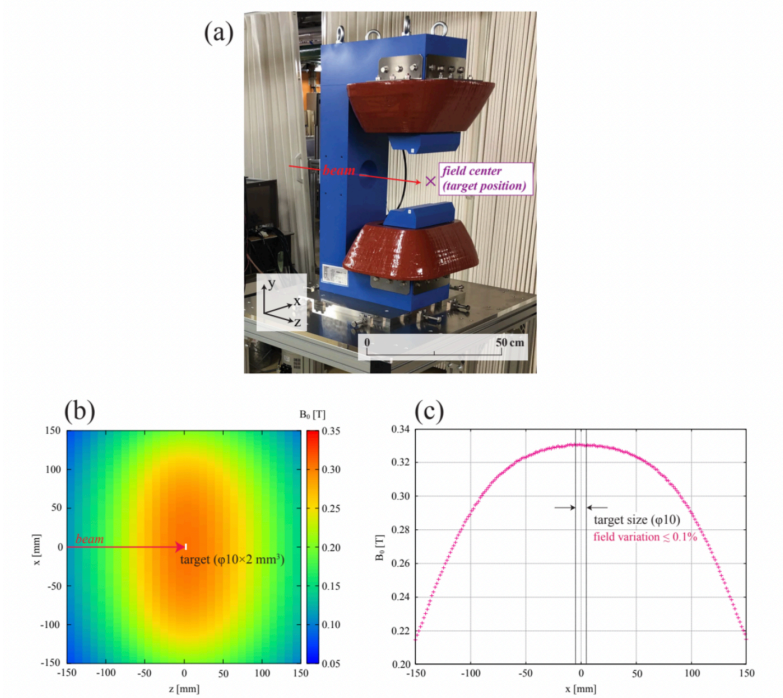
\includegraphics[keepaspectratio, scale=0.8]
       {./chap2/fig/magnet.png}
  \caption{(a)実際の電磁石の写真。(b)80 Aの電流印加時の水平面の磁場強度分布。(c)90 Aの電流印加時のx軸方向の磁場強度分布。標的結晶の中印を原点とする。座標軸はz軸をビームの進行方向としている。標的結晶サイズの範囲における磁場の不均一度は$\leq0.1\%$である。}
  \label{magnet}
 \end{figure}

\subsection{標的チェンバー}
$\ref{chamber_str}$に標的結晶周辺のシステムを示す。標的結晶はテフロン製のサンプルホルダーに
装着し、マイクロ波を効率的に標的に照射するための TE011 型共振器の中心に設置した。
共振器には磁場掃引用のコイルと NMR 測定用のコイルが取り付けられている。また、標
的結晶の角度調整を行うために歯車を用いた回転システムを導入している。
図$\ref{chamber}$に標的チェンバーの模式図を示す。図に示す黒の点線の位置に図$\ref{chamber_str}$のシステム
が導入されている。ナフタレン標的の昇華を防ぐために液体窒素による冷却を行い、冷却による霜
の発生を防止するために真空を引く必要があるため、チェンバーを二重構造とした。


\begin{figure}[ht]
  \centering
  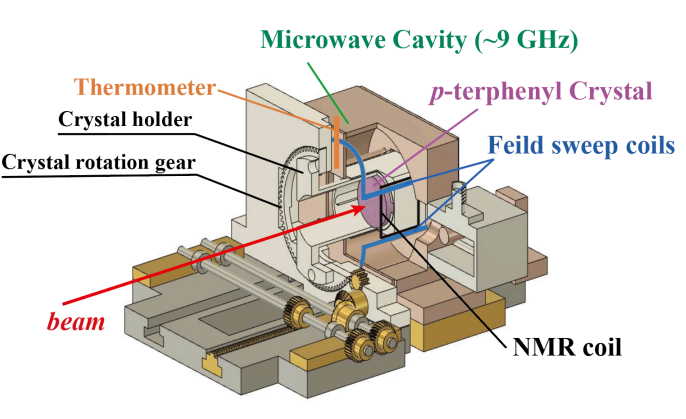
\includegraphics[keepaspectratio, scale=0.8]
       {./chap2/fig/chamber_str.png}
  \caption{標的結晶周辺のシステムの模式図}
  \label{chamber_str}
 \end{figure}

 \begin{figure}[ht]
  \centering
  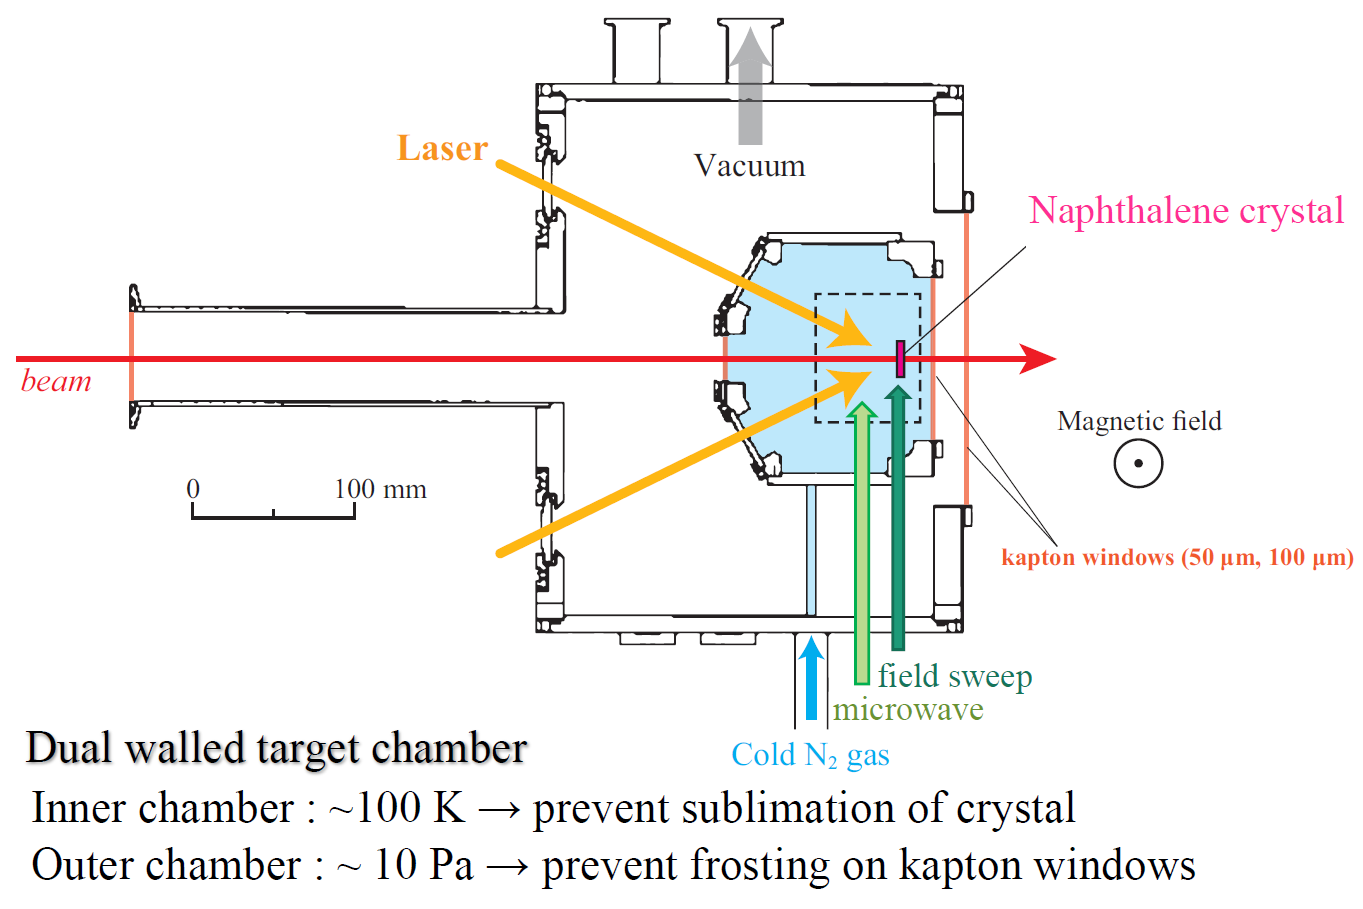
\includegraphics[keepaspectratio, scale=0.5]
       {./chap2/fig/chamber.png}
  \caption{標的チャンバーの模式図。黒の点線内に図$\ref{chamber_str}$のシステムが導入されている}
  \label{chamber}
 \end{figure}

\subsection{パルスレーザ}
パルスレーザは、株式会社 Changchun New Industries Optoelectronics Technology
製の LD 励起固体レーザ(HPL-556-Q-5mJ)を使用した。このレーザは、波長 556 nm、
パルス幅約 600 ns に設定され、最大 5 mJ の単一パルスを発生させることができ、10 Hz
∼ 4 kHz までの繰り返し動作が可能になっている。HIMAC におけるビーム照射試験で
は、パルスの出力を 5 mJ、繰り返し周波数を 1.5 kHz に設定した。図 3.9 に示すように
レーザ光は、加速器実験におけるビームとの干渉を避けるために、標的チェンバーの上流
側に取り付けられた 2 箇所の光学窓から照射される。また、レーザ光の一部はフォトダイ
オードに照射し、TTL 信号に変換してマイクロ波照射と磁場掃引のトリガーに使用した。

\subsection{磁場掃引・マイクロ波回路}
レーザ光をトリガーとし、磁場掃引およびマイクロ波の照射を行うようにした。磁場掃引は、ファンク
ションジェネレーター(NF 社、WF1943A)を用いて三角波(5 Vpp)を生成し、オペア
ンプで増幅後マイクロ波共振器内のコイルに入力した。
マイクロ波は RF オシレータ(SynthHD, Windfreak Tech., LLC)で生成した。そ
の後ファンクションジェネレータ(F.G.)からレーザ光をトリガーとした矩形波を単
極単投(SPST)スイッチに送り、スイッチを制御することでマイクロ波パルスを整形
した。パルス化されたマイクロ波は、RF パワーアンプ(株式会社アールアンドケー、
CA9000BW1G-5060RP)で 400 W まで増幅し、TE011 型共振器へ送った。図$\ref{circuit}$に
Triplet-DNP システムの回路図を示す。

\begin{figure}[ht]
  \centering
  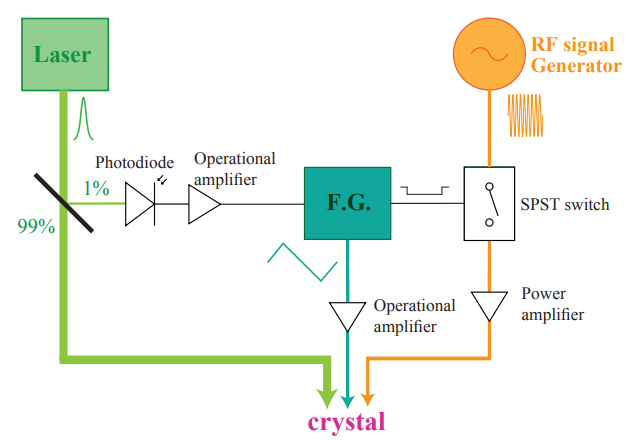
\includegraphics[keepaspectratio, scale=0.8]
       {./chap2/fig/circuit.png}
  \caption{Triplet-DNPシステムの回路図}
  \label{circuit}
 \end{figure}

 \subsection{NMR測定装置}
 NMR 装置の簡潔な回路図を図$\ref{duplexer}$に示す。RF の照射および FID 信号の検出は、デュ
 プレクサを介することで同じ NMR コイルにて行われる。また、NMR 観測シーケンスの
 作成や NMR 信号の受信は OPENCORE NMR 分光計$\cite{Takeda2} $で行っている。回路の共振
 は、チューナーボックス内の可変コンデンサで調節した。

\begin{figure}[ht]
  \centering
  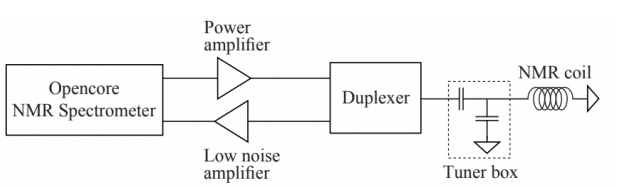
\includegraphics[keepaspectratio, scale=1.0]
       {./chap2/fig/duplexer.png}
  \caption{NMR装置の回路図}
  \label{duplexer}
 \end{figure}


\section{HIMACにおける偏極陽子標的のビーム照射試験}
量子科学技術研究開発機構 HIMAC において、ナフタレン偏極標的に対
して 200 MeV の陽子ビームの照射試験を行った。十分偏極発展が飽和した偏極標的に対
して陽子ビームを照射し、定期的に NMR 測定によって偏極度をモニターすることで放
射損の評価を行った。図 4.6 に 200 MeV の陽子ビーム照射時のナフタレン標的の
NMR 信号強度(FID 信号をフーリエ変換後積分した値)を示す。
この測定では、$1\times10^6$cps のビーム強度で 2 回照射を行い、1 回目では 7.5 h、2 回目
では 10 h 照射した。また 20 分に 1 回の頻度でフリップ角を 12◦ に設定した NMR 測定
を行なった。グラフ$\ref{HIMAC_data}$では、ビーム照射直前の NMR
信号強度を 1 としている。赤色のエリアはビーム照射時であることを示している。
\begin{figure}[ht]
  \centering
  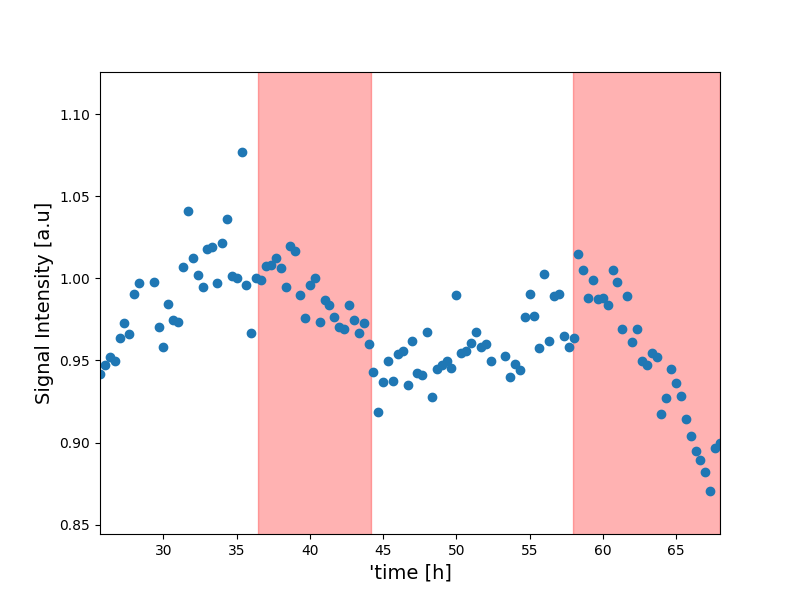
\includegraphics[keepaspectratio, scale=0.7]
       {./chap2/fig/HIMAC_data.png}
  \caption{200 MeV陽子ビーム照射時のナフタレン標的のNMR信号強度。ビーム照射直前のNMR信号強度を1とした。赤色の領域はビーム照射時を示している。}
  \label{HIMAC_data}
 \end{figure}

 グラフ$\ref{HIMAC_data}$に示すようにビーム照射時には偏極度が徐々に低下する
 ことが確認された。

 



% 我々は陽子--$^3$He弾性散乱による$^3$He偏極分解能測定のために、偏極$^3$He標的の開発を行ってきた。この章では、$^3$He原子核の偏極方法とその偏極度の測定方法について記述する。$^3$He原子核の偏極方法としては、スピン交換光ポンピング(Spin Exchange Optical Pumping, SEOP)法を採用した。

% %%%% 2.1 %%%%
%  \section{偏極標的}
% 陽子や中性子の偏極標的は核子のスピン構造の研究に必要不可欠なものである。しかし、陽子に対して自由空間中の中性子は不安定であり、およそ15分の寿命で陽子に$\beta$崩壊してしまう。標的として使用するためには高密度かつ安定である必要があり、現状ではそのような大量の中性子を分離し安定させることは不可能である。偏極中性子標的として原子核物理学や素粒子物理学等において広く開発、利用されているのが偏極$^3$He標的である。$^3$He原子核は2個の陽子と1個の中性子から成り、Pauli原理から陽子はスピン一重項状態となるので、その磁気モーメントは互いに打ち消し合う。よって、$^3$He原子核の正味の磁気モーメントは中性子の磁気モーメントとほぼ等しくなる。また$^3$He原子核の核スピンのおよそ$90$%が中性子のスピンによる寄与であることが示されており\cite{Fri90}、偏極中性子標的として偏極$^3$He標的を実験的に用いることができる。また$^3$He原子核は低エネルギーの中性子に対して、スピンの向きに依存した吸収断面積を持っている\cite{Cou88}。$^3$He原子核スピンと反平行のスピンを持つ中性子に対して大きい吸収断面積を示すので、中性子を偏極させるための偏極子\cite{Cou90}や、偏極した中性子の偏極度計\cite{GTD95}としても利用されている。

% %%%%%%%%%%

% %%%% 2.2 %%%%
%  \section{$^3$He原子核の偏極方法}
% $^3$He原子核を偏極させる方法としては主に二つある。ひとつは準安定交換法(Metastability Exchange Optical Pumping, MEOP)\cite{CSW63}と呼ばれる方法である。これは高周波の放電によって$^3$He原子の電子スピンを$2{}^3S_1$の準安定状態に励起させ、これに1083 nmの円偏光を照射することで$2{}^3P_0$の励起準位へと遷移させる。これによって電子スピンをZeeman分裂した$2{}^3S_1$の特定の副準位へと占有させ、電子スピンを偏極させることができる。この電子スピン偏極は更に基底状態の$^3$He原子核との超微細相互作用によって原子核スピンへと移され、結果的に${}^3$He原子核を偏極させることができる。この反応の断面積は$\sim 10^{-16} \ {\rm cm^2}$と非常に大きいので、高い偏極度を実現できる。しかし、高周波の放電を保持するために$^3$Heガスの圧力を低くする必要があり、およそ数 Torrに制限される。本研究では3気圧程度の$^3$Heガスを想定しているので、この方法は本研究に不適である。\\
%  二つ目は本研究でも採用しているSEOP法\cite{BCV60}である。散乱実験等で必要な高密度の偏極$^3$He標的を実現できるのは現状ではこの方法だけである。SEOP法は主に二つの過程によって$^3$He原子核を偏極させる。最初に、Rb蒸気に円偏光レーザーを照射することでRb原子を偏極させる(光ポンピング)。次に、$^3$He原子核とのスピン交換相互作用によってRb原子の偏極を$^3$He原子核へ移行させる。これらの過程を経て、$^3$He原子核を偏極させる。光ポンピングに数十 W程度の高出力レーザーを用いれば、高密度の$^3$Heガスで高偏極度を実現できる。近年では、$5$気圧程度の圧力で$60$%以上の偏極度が得られている\cite{Ye10}。\\
%  以上より、本研究では$^3$He原子核を偏極させる方法としてSEOP法を採用した。以下の節ではこのSEOP法の原理および高速断熱通過-核磁気共鳴(Adiabatic Fast Passage Nuclear Magnetic Resonance, AFP-NMR)法とRbの電子スピン共鳴(Electron Spin Resonance, ESR)測定による$^3$He原子核の偏極度測定原理について述べる。
% %\textcolor{red}{未}

% %%%%%%%%%%

% %%%% 2.3 %%%%
%  \section{スピン交換光ポンピング法}
%  前述のように、SEOP法は円偏光レーザーによってアルカリ金属原子を偏極させ(光ポンピング)、その偏極した原子と$^3$He原子核とが超微細相互作用(Hyper Fine Interaction, HFI)をすることによってスピン交換が起こり、$^3$He原子核を偏極させる二段階の過程で行う方法である。この節ではこのSEOP法による$^3$He原子核の偏極原理についてそれぞれの過程に分けて述べる。一般的に、光ポンピングにはRb原子が用いられるが、K原子やNa原子、およびそれらの混合蒸気を用いる方法もある\cite{Bab03, Bor03}。本研究では、偏極させるアルカリ金属原子にはRb原子を採用した。

% %% 2.3.1 %%
%   \subsection{光ポンピングによるRb原子の偏極}
%   Rbの同位体は主に$^{85}$Rbと$^{87}$Rbの二種類があり、それらの天然存在比はそれぞれ$72.17%, 27.83%$である。$^{85}$Rbの核スピンは$I=5/2$であり、電子スピンを$S=1/2$、電子の軌道角運動量を$L$、電子の全角運動量を$J=L+S$とすると、Rb原子の全角運動量$F$は$|I-J| \le F \le I+J$の値を取りうる。またそれぞれの$F$の状態は磁気量子数$m_F$について縮退しており、静磁場をかけることによってZeeman分裂する。$^{85}$Rb原子のエネルギー準位を図\ref{85Rb_ene}に示す。
  
% \begin{figure}[tbp]
%  \centering
%  \includegraphics[clip,width=9cm]{./chap2/fig/85Rb_ene_mf.pdf}\\
%  \caption{$^{85}$Rbのエネルギー準位}
%  \label{85Rb_ene}
% \end{figure}
  
%   アルカリ金属原子の偏極には、光子を吸収または放出する際の角運動量選択則を利用している。Rb原子の$D_1$遷移波長(795 nm)の光を入射すると共鳴が起き、Rb原子は$5{}^2S_{1/2}$から$5{}^2P_{1/2}$へと励起する。またこの時、静磁場によってRb原子の準位がZeeman分裂している状態で磁場と平行な右回りの円偏光($\sigma_+$)を入射すると、角運動量選択則により$\Delta m_J=+1$の遷移のみが起こる。よって、$5{}^2S_{1/2}$の準位にいるRb原子の価電子のうち$m_J=-1/2$の準位にいたものだけが$5{}^2P_{1/2}$の$m_J=+1/2$の準位へと選択的に励起される。またこの励起したRb原子は、他の原子が存在しない場合においては$5{}^2S_{1/2}$の$m_J=-1/2$または$m_J=+1/2$状態に脱励起する。この脱励起が起こる確率はClebsch-Gordan係数に従い、それぞれ$2/3, 1/3$となる。この様子を示したのが図\ref{85Rb_ene_pump}である。図ではRb原子の核スピンの影響を無視して簡略化したエネルギー準位を示している。実際にはRb原子の他に最終的に偏極させる3気圧程度の$^3$Heガスや、$\rm N_2$ガスも同時に封入させる。これらの“バッファガス”を混在させると、Rb原子との衝突によって$5{}^2P_{1/2}$の二つの準位($m_J= \pm 1/2$)が混合し(collisional mixing)、$5{}^2S_{1/2}$の二つの準位へとそれぞれ1/2の同確率で脱励起するようになる。円偏光を絶えず入射させれば$5{}^2P_{1/2}$へ励起され続けるので、光子の吸収と脱励起を繰り返し、$5{}^2S_{1/2}$の$m_J=+1/2$状態が占有され、Rb原子を偏極させることができる。
  
% \begin{figure}[tbp]
%  \centering
%  \includegraphics[clip,width=9cm]{./chap2/fig/85Rb_seop.pdf}\\
%  \caption{核スピンの影響を無視した$^{85}$Rbのエネルギー準位および光ポンピングの模式図}
%  \label{85Rb_ene_pump}
% \end{figure}
  
% Rb原子が脱励起する時にも光子が放出される。$m_J=+1/2$状態から$m_J=-1/2$状態への脱励起の場合は右回りの円偏光($\sigma_+$)、$m_J=-1/2$状態から$m_J=+1/2$状態への脱励起の場合は左回りの円偏光($\sigma_-$)の光子が放出され、同じ磁気量子数間での脱励起の場合は非偏光($\pi$)の光子が放出される。脱励起によって放出された光子を吸収することでもRb原子が励起する(radiation trapping)ため、$5{}^2S_{1/2}$の$m_J=+1/2$状態にいるRb原子も励起されてしまい、結果的にRb原子の偏極を飽和させる要因となる。この現象を防ぐために、バッファガスとして$\rm N_2$ガスを封入する。バッファガスを含んだ場合の光ポンピングの模式図を図\ref{85Rb_ene_buf}に示す。円偏光によって励起したRb原子は、$\rm N_2$分子との衝突によってそのエネルギーを$\rm N_2$分子の振動や回転のエネルギーとして渡し、脱励起する。このことによって、光子を放出することなく脱励起させることができる。このとき励起したRb原子が光子を放出して脱励起する確率$B_{\gamma}$は、$\rm N_2$ガスの分圧を$P_{\rm N_2}$とすると、
% %
% \begin{equation}
%  B_{\gamma}=\frac{3}{3+P_{\rm N_2}}
% \end{equation}
% %
% と表される\cite{WC89}。加えられる$\rm N_2$ガスの典型的な分圧は$100 \ \rm Torr$程度であり、このとき光子の放出を伴う遷移が起こる確率はおよそ$3$%にまで抑制される。
  
% \begin{figure}[tbp]
%  \centering
%  \includegraphics[clip,width=9cm]{./chap2/fig/85Rb_seop2.pdf}\\
%  \caption{バッファガス($\rm N_2$)を含んだ場合での光ポンピングの模式図}
%  \label{85Rb_ene_buf}
% \end{figure}

% 次に、以上の条件下におけるRb原子の偏極度の表式を求める。Rb原子の偏極度を$P_{\rm Rb}$とすると、
% %
% \begin{equation}
%  P_{\rm Rb}=\frac{\rho_+ - \rho_-}{\rho_+ + \rho_-}=\rho_+ - \rho_-
%  \label{P_Rb}
% \end{equation}
% %
% となる。$\rho_{\pm}$はRb原子の$m_J= \pm 1/2$における占有確率で、$\rho_+ + \rho_-=1$である。占有確率$\rho_{\pm}$の時間変化は次のように表される\cite{Lar91}。
% %
% \begin{equation}
%  \frac{d\rho_{\pm}(x)}{dt} = \pm \left( \gamma_{\nu}^+(x)+\gamma_{\nu}^0(x)+\Gamma_{\rm Rb}-D\frac{d^2}{dx^2} \right)\rho_-(x) \mp \left( \frac{\Gamma_{\rm Rb}}{2}+\frac{\gamma_{\nu}^0(x)}{2} \right)
%  \label{rho_Rb}
% \end{equation}
% %
% ここで、$\gamma_{\nu}^{+, 0}(x)$は位置$x$での円偏光($\sigma_+$)および直線偏光の光子がRb原子に吸収される割合で、$\Gamma_{\rm Rb}$はRb原子の偏極緩和率、$D$は$^3$Heガス中でのRb原子に対する有効拡散定数で、ガスが封入されているセルの境界付近でのRb原子の偏極度およびガスの非一様性の効果を表している。レーザー光が完全に円偏光している場合は$\gamma_{\nu}^0(x)=0$である。またガスが十分高圧、高密度であれば占有確率$\rho_{\pm}(x)$はセル内でほぼ一様と考えられるので、
% %
%  \begin{equation}
%   -D \frac{d^2}{dx^2} \rho_-(x) \ll 1
%  \end{equation}
% %
% と近似できる。よって式(\ref{rho_Rb})は以下のように単純化される。
% %
% \begin{eqnarray}
%  \frac{d\rho_{\pm}(x)}{dt} & = & \pm \left( \gamma_{\nu}^+(x)+\Gamma_{\rm Rb} \right) \rho_-(x) \mp \frac{\Gamma_{\rm Rb}}{2} \nonumber \\
%  & = & \pm \left( \gamma_{\nu}^+(x)+ \frac{\Gamma_{\rm Rb}}{2} \right) \rho_-(x) \mp \frac{\Gamma_{\rm Rb}}{2}\rho_+(x)
%  \label{drho/dt}
% \end{eqnarray}
% %
% 式(\ref{P_Rb}), (\ref{drho/dt})より、Rb原子の偏極度$P_{\rm Rb}$の時間変化は次のように表される。
% %
% \begin{eqnarray}
%  \frac{dP_{\rm Rb}(x)}{dt} & = & \frac{d}{dt}(\rho_+(x)-\rho_-(x)) \nonumber \\
%  & = & -\left( \gamma_{\nu}^+(x)+\Gamma_{\rm Rb} \right) P_{\rm Rb}(x)+\gamma_{\nu}^+(x)
% \end{eqnarray}
% %
% この微分方程式を解くと、結局Rb原子の偏極度は
% %
% \begin{equation}
%  P_{\rm Rb}(x, t) = \left( \frac{\gamma_{\nu}^+(x)}{\gamma_{\nu}^+(x)+\Gamma_{\rm Rb}} \right) \left[ 1-e^{-(\gamma_{\nu}^+(x)+\Gamma_{\rm Rb})t} \right]
%  \label{P_Rb_xt}
% \end{equation}
% %
% と書ける。十分な時間円偏光による光ポンピングを行い平衡状態に達したと仮定すると、この時のRb原子の偏極度$\overline{P}_{\rm Rb}$は、式(\ref{P_Rb_xt})の$t \to \infty$の極限を取って
% %
% \begin{equation}
%  \overline{P}_{\rm Rb}(x) = \frac{\gamma_{\nu}^+(x)}{\gamma_{\nu}^+(x)+\Gamma_{\rm Rb}}
%  \label{P_Rb_ave}
% \end{equation}
% %
% となる。すなわち、Rb原子の偏極度は光ポンピングによる円偏光($\sigma^+$)の光子の吸収率$\gamma_{\nu}^+(x)$とRb原子の偏極緩和率$\Gamma_{\rm Rb}$の比で表される。\\
%  円偏光($\sigma^+$)の光子の吸収率$\gamma_{\nu}^+(x)$は次のように表される。
% %
% \begin{equation}
%  \gamma_{\nu}^+(x) = \int \Phi(x, \nu) \sigma_{\rm abs}(\nu) d\nu
%  \label{gam+}
% \end{equation}
% %
% ここで$\Phi(x, \nu)$は位置$x$における単位周波数あたりの円偏光($\sigma^+$)光子の光束であり、$\sigma_{\rm abs}(\nu)$は周波数$\nu$の光子に対する吸収断面積である。\\
%  光子はRb蒸気中を進むにつれ吸収され数が減少していくため、円偏光光子の光束$\Phi(x, \nu)$は$x$方向に対して以下のような関係を持つ。
% %
% \begin{eqnarray}
%  \Phi(0, \nu) &=& \frac{I_{\rm laser}(\nu)}{h\nu} \\
%  \frac{d\Phi(x, \nu)}{dx} &=& -[{\rm Rb}] \sigma_{\rm abs}(\nu) (1-P_{\rm Rb}(x)) \Phi(x, \nu)
% \end{eqnarray}
% %
% ここで、$I_{\rm laser}(\nu)$は円偏光レーザーの単位周波数および単位面積あたりの出力で、$h$はPlanck定数である。\\
%  吸収断面積$\sigma_{\rm abs}(\nu)$は次の式で表される\cite{Lar91}。
% %
% \begin{equation}
%  \sigma_{\rm abs}(\nu) = \frac{\lambda_0^2}{8\pi}\Gamma_{\rm nat} \left[ \frac{\Gamma}{(\nu-\nu_0)^2+(\Gamma/2)^2}+\frac{b(\nu-\nu_0)}{\Gamma} e^{-\frac{|\nu-\nu_0|}{\Gamma_a}} \right]
%  \label{sig_abs}
% \end{equation}
% %
% ここで$\lambda_0=794.979~{\rm nm}$、$\nu_0=c/\lambda_0$はそれぞれRb原子の$D_1$遷移波長および周波数であり、$\Gamma_{\rm nat}=5.75~{\rm MHz}$は自然線幅である。$\Gamma$はバッファガスによる全圧力拡がり幅で、$b$および$\Gamma_a$は観測された吸収スペクトルの非対称を説明するための補正係数である。これらの値はLarsonらによって測定されており、それぞれの値は表\ref{par_abs}のようになる。またバッファガスとして$2.94$気圧の$^3$Heガスが存在する時のRb原子の光子吸収断面積$\sigma_{\rm abs}$を図\ref{sig_abs_Rb}に示す。

% \begin{table}[htbp]
%  \caption{Rbの$D_1$線遷移に対する光子吸収の係数\cite{Lar91}}
%  \centering
%  \begin{tabular}{|c|ccc|} \hline
%   $^3$He圧力 [atm] & $\Gamma$ [GHz] & $\Gamma_a$ [GHz] & $b$ [$10^{-12}$ s] \\ \hline \hline
%   2.94 & $54 \pm 3$ & $154 \pm 11$ & $0.20 \pm 0.04$ \\
%   6.44 & $126 \pm 5$ & $146 \pm 11$ & $1.0 \pm 0.2$ \\ 
%   8.97 & $184 \pm 6$ & $184 \pm 11$ & $1.5 \pm 0.2$ \\
%   12.1 & $244 \pm 7$ & $225 \pm 12$ & $1.5 \pm 0.2$ \\ \hline
%  \end{tabular}
%  \label{par_abs}
% \end{table}

% \begin{figure}[tbp]
%  \centering
%  \includegraphics[clip,width=10cm]{./chap2/fig/sigma_abs.eps}\\
%  \caption{Rb原子の$D_1$遷移の光子吸収断面積}
%  \label{sig_abs_Rb}
% \end{figure}

% 次に、Rb原子の偏極緩和率$\Gamma_{\rm Rb}$の表式を求める。Rb原子の偏極緩和の主な要因は、Rb原子と他の原子が衝突することによって起こるスピン-回転相互作用である\cite{WWH85}。このスピン-回転相互作用のハミルトニアンは以下のように書ける。
% %
% \begin{equation}
%  \mathcal{H}_{\rm SR} = \gamma {\bm N} \cdot {\bm S}
% \end{equation}
% %
% ここで$\gamma$は結合定数、$\bm N$は衝突した二つの粒子による回転運動の角運動量ベクトルであり、$\bm S$はRb原子の価電子スピンである。一般的に、光ポンピングに用いられる混合気体にはRb、$^3$HeおよびN$_2$が含まれるので、偏極したRb原子は主にこれらの原子との相互作用によって緩和する。よって、Rb原子の偏極緩和率$\Gamma_{\rm Rb}$は混合気体中の各原子の数密度に比例し、次の式で表される\cite{Lar91,WC94}。
% %
% \begin{equation}
%  \Gamma_{\rm Rb} = \langle \sigma_{\rm SD} v \rangle [{\rm Rb}]+\langle \sigma_{\rm N_2} v \rangle [{\rm N_2}]+\langle \sigma_{\rm SE} v \rangle [^3{\rm He}]+k_3 [^3{\rm He}]^2
%  \label{relax_Rb}
% \end{equation}
% %
% ここで、$\langle \sigma v \rangle$は二粒子間の反応断面積$\sigma$および相対速度$v$の積を速度分布で平均化した反応率である。$\sigma_{\rm SD}$はRb同士での反応断面積で、$\sigma_{\rm N_2}$はRb-N$_2$間、$\sigma_{\rm SE}$はRb-$^3$He間での反応断面積である。$k_3$はRbと二つの$^3$Heによる三体衝突における反応率である。また式中の[ ]は各原子または分子の数密度を表す。各反応率はWagshulとChupp\cite{WC94}やLarsonら\cite{Lar91}によって求められており、それぞれの値は以下のようになる。
% %
% \begin{eqnarray}
%  \langle \sigma_{\rm SD} v \rangle &=& (8.3 \pm 0.6) \times 10^{-13}~[{\rm cm^3/s}] \\
%  \langle \sigma_{\rm N_2} v \rangle &=& (9.38 \pm 0.22) \times 10^{-18}~[{\rm cm^3/s}] \\
%  \langle \sigma_{\rm SE} v \rangle &=& (6.1 \pm 0.2) \times 10^{-20}~[{\rm cm^3/s}] \\
%  k_3 &\sim& 7.48 \times 10^{-39}~[{\rm cm^6/s}]
% \end{eqnarray}
% %
% これらの値から、Rb原子の偏極緩和率$\Gamma_{\rm Rb}$を概算する。$^3$Heの密度は$0~℃$、$1$気圧下で$1.35 \times 10^{-4}~{\rm g/cm^3}$であり、$^3$He原子の原子量は$3.015~{\rm g/mol}$である。またN$_2$分子の密度は$0~℃$、$1$気圧下で$1.25 \times 10^{-3}~{\rm g/cm^3}$であり、またN$_2$分子の分子量は$28.01~{\rm g/mol}$である。$^3$Heガスの圧力を$3$気圧、N$_2$ガスの圧力を$100~{\rm Torr}$とすると、それぞれの数密度は室温($300~{\rm K}$)においては
% %
% \begin{eqnarray}
%  [^3{\rm He}] &\simeq& 7.36 \times 10^{19}~[{\rm cm^{-3}}]
%  \label{[3He]} \\
%  {[{\rm N_2}]} &\simeq& 3.20 \times 10^{18}~[{\rm cm^{-3}}]
%  \label{[N2]}
% \end{eqnarray}
% %
% となる。またRb原子の数密度については、Killianによって温度に対するRbの飽和蒸気圧が測定されており\cite{Kil26}、絶対温度$T$におけるRb原子の飽和密度は
% %
% \begin{equation}
%  [{\rm Rb}] = 10^{26.41-\frac{4132}{T}-\log_{10}T}~[{\rm cm^{-3}}]
%  \label{Killian_eq}
% \end{equation}
% %
% と表される。式(\ref{Killian_eq})より、$200$℃におけるRb原子の数密度は
% %
% \begin{equation}
%  [{\rm Rb}] \simeq 10.05 \times 10^{14}~[{\rm cm^{-3}}]
% \end{equation}
% %
% と求められる。よって、以上の条件下におけるRb原子の偏極緩和率$\Gamma_{\rm Rb}$は、式(\ref{relax_Rb})にこれらの値を代入して
% %
% \begin{equation}
%  \Gamma_{\rm Rb} \simeq 909~[{\rm s^{-1}}]
% \end{equation}
% %
% となる。
% %%%%%%%

% %% 2.3.2 %%
%   \subsection{スピン交換による$^3$He原子核の偏極}
% Rb蒸気と$^3$Heガスが混在した空間では、Rb原子の価電子と$^3$He原子核の間で超微細相互作用(HFI)が起こり、それによってRb原子の偏極が$^3$He原子核へと移行する(スピン交換)。HFIによるスピン交換の概念図を図\ref{spin_exch}に示す。Rb原子の価電子と$^3$He原子核とのHFIにおけるハミルトニアンは次の式で表される\cite{Her65}。
% %
% \begin{equation}
%  \mathcal{H}_{\rm HFI} = -2 \gamma_{\rm ^3He} \mu_{\rm N} \mu_{\rm B} \sum_{i=1}^3 \left[ \frac{{\bm I} \cdot {\bm J}_i}{r_i^3} - 3\frac{({\bm I} \cdot {\bm r}_i)({\bm J}_i \cdot {\bm r}_i)}{r_i^5} - \frac{8\pi}{3} \delta({\bm r}_i) {\bm I} \cdot {\bm J}_i \right]
% \end{equation}
% %
% ここで、$\gamma_{\rm ^3He}$は$^3$Heの磁気回転比であり、$\mu_{\rm N}$は核磁気モーメント、$\mu_{\rm B}$はBohr磁子である。$\bm I$は$^3$He原子核の核スピンで、${\bm J}_i$は$i$番目の電子のスピンである。${\bm r}_i$は$^3$He原子核から見た$i$番目の電子に対する位置ベクトルであり、$i=1$はRb原子の価電子、$i=2,3$は$^3$Heの電子を表す。また$ \delta({\bm r}_i)$は三次元デルタ関数である。括弧内の第一項および第二項は二粒子間での磁気双極子相互作用を表し、第三項はFermi接触相互作用を表す項である。

% \begin{figure}[tbp]
%  \centering
%   \includegraphics[width=9cm]{./chap2/fig/spin_exchange.pdf}\\
%  \caption{Rb原子と$^3$He原子核のスピン交換反応の概念図}
%  \label{spin_exch}
% \end{figure}

% 次に、$^3$He原子核の偏極度の表式を求める。静磁場中の$^3$He原子核はRb原子と同様に磁気量子数$m_I=\pm 1/2$についてZeeman分裂する。この分裂した二つの副準位それぞれの占有確率を$\tilde{\rho}_{\pm}~(\tilde{\rho}_+ + \tilde{\rho}_- =1)$とすると、$^3$He原子核の偏極度は
% %
% \begin{equation}
%  P_{\rm ^3He} = \frac{\tilde{\rho}_+ - \tilde{\rho}_-}{\tilde{\rho}_+ + \tilde{\rho}_-} = \tilde{\rho}_+ - \tilde{\rho}_-
%  \label{P_3He}
% \end{equation}
% %
% と表される。占有確率$\tilde{\rho}_{\pm}$の時間変化は次の式で表される\cite{Lar91}。
% %
% \begin{equation}
%  \frac{d\tilde{\rho}_{\pm}}{dt} = \pm \left( \frac{\Gamma_{\rm ^3He}}{2} + \gamma_{\rm SE}\rho_+ \right) \tilde{\rho}_- \mp \left( \frac{\Gamma_{\rm ^3He}}{2} + \gamma_{\rm SE}\rho_- \right) \tilde{\rho}_+
%  \label{drho/dt_3He}
% \end{equation}
% %
% ここで、$\gamma_{\rm SE}$はRb原子と$^3$He原子核のスピン交換率で、$\Gamma_{\rm ^3He}$は$^3$He原子核の偏極緩和率である。スピン交換率$\gamma_{\rm SE}$はRb原子の数密度に比例し、
% %
% \begin{equation}
%  \gamma_{\rm SE} = \langle  \sigma_{\rm SE} v \rangle [{\rm Rb}] \equiv k_{\rm SE} [{\rm Rb}]
% \end{equation}
% %
% と書ける。$k_{\rm SE}$はスピン交換率係数であり、Larsonら\cite{Lar91}やChannら\cite{Cha02}によって測定されている。それぞれの値は$(6.1 \pm 0.2) \times 10^{-20}~{\rm cm^3/s}$ \cite{Lar91}, $(6.8 \pm 0.2) \times 10^{-20}~{\rm cm^3/s}$ \cite{Cha02}と求められている。\\
%  $\tilde{\rho}_+ + \tilde{\rho}_- =1$より、式(\ref{drho/dt_3He})を整理すると、結局$^3$He偏極度の時間変化は次のように表される。
% %
% \begin{equation}
%  \frac{dP_{\rm ^3He}}{dt} = -(\gamma_{\rm SE}+\Gamma_{\rm ^3He}) P_{\rm ^3He} + \gamma_{\rm SE} \overline{P}_{\rm Rb}
%  \label{dP_3He/dt}
% \end{equation}
% %
% ここで、Rb原子の偏極度$P_{\rm Rb}$は$^3$He原子核の偏極度$P_{\rm ^3He}$に比べて十分早く平衡状態に達すると仮定し、$\overline{P}_{\rm Rb} \sim \rho_+ - \rho_-$とした。式(\ref{dP_3He/dt})を解くと、結局$^3$He原子核の偏極度$P_{\rm ^3He}$は以下の式で表される。
% %
% \begin{equation}
%  {P}_{\rm ^3He} = \overline{P}_{\rm Rb} \frac{\gamma_{\rm SE}}{\gamma_{\rm SE}+\Gamma_{\rm ^3He}} \left[ 1-e^{-(\gamma_{\rm SE}+\Gamma_{\rm ^3He})t} \right]
%  \label{P_3He_final}
% \end{equation}
% %
% 式(\ref{P_3He_final})より、十分時間が経過した時($t \to \infty$)の$^3$He原子核の偏極度$\overline{P}_{\rm ^3He}$は
% %
% \begin{equation}
%  \overline{P}_{\rm ^3He} = \overline{P}_{\rm Rb} \frac{\gamma_{\rm SE}}{\gamma_{\rm SE}+\Gamma_{\rm ^3He}}
%  \label{P_3He_ave}
% \end{equation}
% %
% と表される。また式(\ref{P_Rb_ave})より
% %
% \begin{equation}
%  \overline{P}_{\rm ^3He} = \frac{\gamma_{\nu}^+(x)}{\gamma_{\nu}^+(x)+\Gamma_{\rm Rb}} \frac{\gamma_{\rm SE}}{\gamma_{\rm SE}+\Gamma_{\rm ^3He}}
%  \label{P_3He_ave2}
% \end{equation}
% %
% となる。よって、$^3$He原子核の偏極度を向上させるためには、円偏光光子の吸収率$\gamma_{\nu}^+$をなるべく大きくしつつ、Rb原子の偏極緩和率$\Gamma_{\rm Rb}$を小さくすることでRb原子の偏極度$\overline{P}_{\rm Rb}$を向上させることが必要である。またスピン交換率$\gamma_{\rm SE}$をなるべく大きくしつつ、$^3$He原子核の偏極緩和率$\Gamma_{\rm ^3He}$を小さくすることも必要である。これらのパラメーターはRb原子の数密度$[{\rm Rb}]$に依存し、また$[{\rm Rb}]$は式(\ref{Killian_eq})より温度依存性を持つので、$^3$He原子核の偏極度を向上させるためにはRb蒸気の温度を最適化することが重要である。\\
%  次に、$^3$He原子核の偏極緩和率$\Gamma_{\rm ^3He}$について述べる。$^3$He原子核の偏極緩和の原因は主に以下の3つである。
% %
% \begin{enumerate}
%  \item $^3$He原子核同士の磁気双極子相互作用による緩和($\Gamma_D$)
%  \item 静磁場の不均一度による緩和($\Gamma_B$)
%  \item ガラスセル内に含まれる不純物やセルの内壁との接触による緩和($\Gamma_W$)
% \end{enumerate}
% %
% $^3$He原子核の偏極緩和率$\Gamma_{\rm ^3He}$はこれらの和で表される。以下に、それぞれの緩和の原因について述べる。\\
%  $^3$He原子核同士の磁気双極子相互作用による偏極緩和率$\Gamma_D$は、Newburyらによって計算されており、
% %
% \begin{equation}
%  \Gamma_D = \frac{[{\rm ^3He}]}{744}~[{\rm h}^{-1}]
% \end{equation}
% %
% と表される\cite{New93}。ここで、$^3$Heの数密度$[{\rm ^3He}]$の単位はamagat($1 {\rm amg} = 2.689 \times 10^{19}~{\rm cm^{-3}}$)である。$3$気圧、$300~{\rm K}$の$^3$Heガスを仮定すると、式(\ref{[3He]})より$[{\rm ^3He}]$はamagat単位において
% %
% \begin{equation}
%  [{\rm ^3He}] = \frac{7.36 \times 10^{19}}{2.689 \times 10^{19}} \simeq 2.74~[{\rm amg}]
% \end{equation}
% %
% となる。よって、$\Gamma_D$は
% %
% \begin{equation}
%  \Gamma_D = \frac{2.74}{744} \simeq 3.68 \times 10^{-3}~[{\rm h^{-1}}]
%  \label{Gam_D}
% \end{equation}
% %
% と計算できる。\\
%  静磁場の不均一度による偏極緩和率$\Gamma_B$は次の式で表される\cite{CSH88}。
% %
% \begin{equation}
%  \Gamma_B = D_{\rm ^3He} \frac{|\nabla B_x|^2+|\nabla B_y|^2}{B_z^2}
%  \label{Gam_B}
% \end{equation}
% %
% ここで、$D_{\rm ^3He}$は偏極した$^3$He核スピンの拡散定数であり、$B_x,~B_y,~B_z$は静磁場の各軸成分である。偏極した$^3$He核スピンの拡散定数$D_{\rm ^3He}$は、GamblinとCarverによって次の式で表されることが示されている\cite{GC65}。
% %
% \begin{equation}
%  D_{\rm ^3He} = \frac{1}{2.13} \frac{\lambda v}{(1+ \omega^2 \tau^2)}
%  \label{D_3He}
% \end{equation}
% %
% ここで、$\lambda$および$v$は$^3$He原子の平均自由行程と二乗平均速度($\sqrt{\langle v^2 \rangle}$)である。また$\omega$は$^3$He核スピンのLarmor歳差運動周波数で、$\tau = \lambda/v$は$^3$Heガスの衝突時間である。圧力$p$、温度$T$の気体における平均自由行程$\lambda$は、次のように書ける。
% %
% \begin{equation}
%  \lambda = \frac{k_{\rm B}T}{\sqrt{2} \sigma p}
%  \label{MFP}
% \end{equation}
% %
% ここで、$k_{\rm B}$はBoltzmann定数であり、$\sigma$は気体粒子の幾何学的断面積である。気体粒子が半径$r$の剛体球だとすれば$\sigma = 4 \pi r^2$と書けるので、半径$r$としてHeのVan der Waals半径($1.40~$\AA)を用いると、結局$3$気圧、$300~{\rm K}$の$^3$Heガスにおける平均自由行程$\lambda$は
% %
% \begin{eqnarray}
%  \lambda &=& \frac{1.38 \times 10^{-23} \cdot 300}{\sqrt{2} \cdot 4 \pi \cdot (1.40 \times 10^{-10})^2 \cdot 3 \times 1.013 \times 10^5} \nonumber \\
%  &\simeq& 3.91 \times 10^{-8}~[{\rm m}]
%  \label{MFP_cal}
% \end{eqnarray}
% %
% となる。二乗平均速度$v$は、気体粒子がMaxwellの速度分布に従っているとすると、
% %
% \begin{equation}
%  v = \left( \frac{3k_{\rm B}T}{m} \right)^{\frac{1}{2}}
%  \label{MSV}
% \end{equation}
% %
% と書ける。$^3$He原子の質量は$2809~{\rm MeV}$なので、$3$気圧、$300~{\rm K}$の$^3$Heガスにおける二乗平均速度$v$は
% %
% \begin{eqnarray}
%  v &=& \left( \frac{3 \cdot 1.38 \times 10^{-23} \cdot 300}{2809 \times 10^6 \div (3.0 \times 10^8)^2 \cdot 1.6 \times 10^{-19}} \right)^{\frac{1}{2}} \nonumber \\
%  &\simeq& 1.58 \times 10^3~[{\rm m/s}]
%  \label{MSV_cal}
% \end{eqnarray}
% %
% となる。$^3$He核スピンのLarmor歳差運動周波数$\omega$は、$^3$Heの磁気回転比を$\gamma_{\rm ^3He}$とすると次の式で表される。
% %
% \begin{equation}
%  \omega = |\gamma_{\rm ^3He}| B_0
%  \label{Larmor-freq}
% \end{equation}
% %
% $^3$Heガスが$B_0 = 2~{\rm mT}$の静磁場中にあるとし、また$\gamma_{\rm ^3He} = -2.04 \times 10^5~{\rm rad \cdot s^{-1} \cdot mT^{-1}}$であるから、$^3$He核スピンのLarmor歳差運動周波数$\omega$は
% %
% \begin{equation}
%  \omega = 2.04 \times 10^5 \cdot 2 = 4.08 \times 10^5~[{\rm s^{-1}}]
%  \label{Larmor-freq_cal}
% \end{equation}
% %
% となる。これらの値を式(\ref{D_3He})に代入すると、偏極した$^3$He核スピンの拡散定数$D_{\rm ^3He}$は次のように求められる。
% %
% \begin{eqnarray}
%  D_{\rm ^3He} &=& \frac{1}{2.13} \frac{3.91 \times 10^{-8} \cdot 1.58 \times 10^3}{\left[ 1+ (4.08 \times 10^5)^2 \left( \dfrac{3.91 \times 10^{-8}}{1.58 \times 10^3} \right)^2 \right]} \nonumber \\
%  &\simeq& 2.90 \times 10^{-5}~[{\rm m^2/s}] \nonumber \\
%  &\simeq& 1.04 \times 10^3~[{\rm cm^2/h}]
%  \label{D_3He_cal}
% \end{eqnarray}
% %
% よって、静磁場の不均一度が$10^{-3}~{\rm cm^{-1}}$程度ならば、静磁場の不均一度による$^3$Heの偏極緩和率$\Gamma_B$は
% %
% \begin{eqnarray}
%  \Gamma_B &\sim& 1.04 \times 10^3 \cdot (10^{-3})^2 \nonumber \\
%  &=& 1.04 \times 10^{-3}~[{\rm h^{-1}}]
%  \label{Gam_B_cal}
% \end{eqnarray}
% %
% となり、$^3$He原子核同士の磁気双極子相互作用による偏極緩和率$\Gamma_D$と同程度の値となる。\\
%  最後に、ガラスセル内に含まれる不純物やセルの内壁との接触による偏極緩和率$\Gamma_W$について述べる。この偏極緩和は、ガラスに含まれる強磁性体や水、油脂等の有機物、空気中の酸素等との相互作用によるものである。これらを抑制するためには、強磁性体の含有量が少ないガラス素材の使用、ガラスセルの洗浄による強磁性体や有機物の除去、またガラスセルを数$100$℃の高温に熱すること(ベーキング)による水や有機物の除去といった対策を取ることが必要である。更にガラスセルに導入する$^3$HeガスやN$_2$ガスの純度を高めるために純化装置を通過させてから導入することも重要である。\\
%  これらの偏極緩和率はRb原子の数密度$[{\rm Rb}]$に依存しないので、それらの和である$\Gamma_{\rm ^3He}$はガラスセル内の温度を常温にすることで測定できる(この測定についての詳細は下記参照)。過去に我々のグループが製作したガラスセルにおける典型的な値は$\Gamma_{\rm ^3He} \sim 0.1~[{\rm h^{-1}}]$であり、偏極緩和の要因はガラスセル内の不純物によるものが支配的であることが分かっている。\\
%  以上の偏極緩和に加え、Channらの実験グループによってRb原子の数密度$[{\rm Rb}]$に比例した“余剰な”偏極緩和があることが報告されている\cite{Cha03}。Channらは実験で得られたRb原子の数密度$[{\rm Rb}]$に対する$^3$He原子核の偏極度を再現するために、式(\ref{P_3He_ave})を以下のように修正している。
% %
% \begin{equation}
%  \overline{P}_{\rm ^3He} = \overline{P}_{\rm Rb} \frac{\gamma_{\rm SE}}{\gamma_{\rm SE}(1+X)+\Gamma_{\rm ^3He}}
%  \label{P_3He_X}
% \end{equation}
% %
% ここで、$X$は$X$-factorと呼ばれる現象論的パラメーターである。$X$-factorはガラスセルの形状によって様々な値を取ることが知られており、ガラスセルの表面積$S$と体積$V$の比$S/V$と相関を持つことが示唆されている\cite{Bab06}。我々のグループが製作したガラスセルでの典型的な値は$X \sim 0.6$である\cite{shiokawa}。

% %%%%%%%
% %%%%%%%%%%

% %%%% 2.4 %%%%
%  \section{AFP-NMR法による$^3$He偏極度測定}
% 陽子--$^3$He弾性散乱実験における$^3$He偏極分解能を測定によって得るためには、実験中の$^3$He原子核の偏極度を知る必要がある。そこで我々のグループは、$^3$He原子核の偏極度の測定方法として、高速断熱通過-核磁気共鳴(AFP-NMR)法を採用した。AFP-NMR法は、偏極した粒子集団の偏極方向を偏極を壊すことなく変化させる方法である。$^3$He原子核の核スピンは$1/2$であり、磁気量子数$m_I=+1/2$の状態に占有している粒子集団をAFP-NMR法によって$m_I=-1/2$の状態へと変化させることができる。これによって、$^3$He原子核の偏極方向を反転できる。反転する偏極した粒子集団によって作られる巨視的な磁化を測定することによって、$^3$He原子核の偏極度を得られる。本節では、このAFP-NMR法の原理について述べる。\\
%  偏極した$^3$He原子核集団が作る磁化を$\bm M$とすると、静磁場$\bm B$中においては磁化$\bm M$はトルク$\bm M \times \bm B$を受け歳差運動をするので、その運動方程式は次のように書ける。
% %
% \begin{equation}
%  \frac{d \bm M}{dt} = \gamma_{\rm ^3He} \bm M \times \bm B
% \end{equation}
% %
% この歳差運動を角速度$\omega$を持つ回転座標系から見た場合を考える。静止座標系から回転座標系への変換は、任意のベクトルを$\bm A$とすると
% %
% \begin{equation}
%  \frac{d \bm A}{dt} = \frac{d^* \bm A}{dt} + \bm \omega \times \bm A
% \end{equation}
% %
% と表される。ここで、$d^*/dt$は回転座標系における時間微分であり、$\bm \omega$は角速度ベクトルである。よって、回転座標系における磁化$\bm M$の運動方程式は
% %
% \begin{equation}
%  \frac{d^* \bm M}{dt} = \gamma_{\rm ^3He} \bm M \times \left( \bm B + \frac{\bm \omega}{\gamma_{\rm ^3He}} \right)
% \end{equation}
% %
% となる。すなわち、回転座標系において磁化$\bm M$が感じる有効磁場$\bm B_{\rm eff}$は、$\bm B_{\rm eff} = \bm B + \bm \omega / \gamma_{\rm ^3He}$となる。\\
%  角速度ベクトル$\bm \omega$は静磁場$\bm B$に平行で、どちらも$z$軸方向を向いているとする($\bm \omega = \omega \bm e_z,~\bm B = B \bm e_z$)。この時、静止系において$z$軸方向に対して垂直な方向に周波数$\omega$の振動磁場$\bm B_1 = 2B_1 \cos (\omega t) \bm e_x$を印加した場合を考える。この振動磁場$\bm B_1$は次のように$xy$平面を互いに反対方向に回転する二つの回転磁場に分解できる。\\
% %
% \begin{equation}
%  \bm B_1 = \left(
%   \begin{array}{c}
%    2B_1 \cos (\omega t)\\ 0\\ 0
%   \end{array}
%  \right) = \left(
%   \begin{array}{c}
%    B_1 \cos (\omega t)\\ B_1 \sin (\omega t)\\ 0
%   \end{array}
%  \right) + \left(
%   \begin{array}{c}
%    B_1 \cos (-\omega t)\\ B_1 \sin (-\omega t)\\ 0
%   \end{array}
%  \right)
% \end{equation}
% %
% 二つの回転磁場のうち回転座標系と同じ方向に回転する磁場成分のみを考えると、偏極した$^3$He原子核集団が作る磁化$\bm M$が感じる有効磁場は
% %
% \begin{equation}
%  \bm B_{\rm eff} = \left( B + \frac{\omega}{\gamma_{\rm ^3He}} \right) \bm e_z + B_1 \bm e'_x
% \end{equation}
% %
% となる。ここで、$\bm e'_x = \bm e_x \cos (\omega t) + \bm e_y \sin (\omega t)$は回転座標系における座標軸方向の単位ベクトルである。よって、静磁場$\bm B$の大きさ$B$を
% %
% \begin{equation}
%  B \equiv B_0 = - \frac{\omega}{\gamma_{\rm ^3He}} = - \frac{2 \pi f}{\gamma_{\rm ^3He}}
%  \label{B0_reso}
% \end{equation}
% %
% を横切るようにして十分大きい値から小さい値へと掃引することで、回転座標系における有効磁場を反転させることができる。ここで、$f$は周波数である。これにより、偏極した$^3$He原子核集団の偏極方向も反転させることができる。有効磁場の反転の概念図を図\ref{afp_sche}に示す。

% \begin{figure}[tbp]
%  \centering
%   \includegraphics[width=11cm]{./chap2/fig/afp_sche.pdf}\\
%  \caption{AFP-NMR法による有効磁場の反転の概念図}
%  \label{afp_sche}
% \end{figure}

% 次に、偏極した$^3$He原子核集団の偏極方向を反転させるために満たすべき条件(AFP条件)について述べる。AFP条件は、断熱条件、高速条件、反転条件の三つから成る。以下に、それぞれの条件について述べる。
% %
% \begin{enumerate}
%  \item {\bf 断熱条件}\\
%  有効磁場の時間変化率は$^3$He原子核のスピンがそれに追従できる程度に遅い必要がある。すなわち、磁化$\bm M$の歳差運動の軸である有効磁場$\bm B_{\rm eff}$の傾く速さが、磁化の歳差運動の周波数よりも十分遅くなければならない。よって、
% %
% \begin{equation}
%  \frac{1}{B_{\rm eff}} \frac{dB_{\rm eff}}{dt} \ll |\gamma_{\rm ^3He}| B_{\rm eff}
%  \label{adia-con}
% \end{equation}
% %
% を満たす必要がある。ここで、$B_{\rm eff} = |\bm B_{\rm eff}|$である。$B = B_0$では、有効磁場の大きさ$B_{\rm eff}$の時間変化率は最も大きくなり、その大きさは最も小さくなるので、式(\ref{adia-con})は以下のように書き換えられる。
% %
% \begin{equation}
%  \frac{1}{B_1} \frac{dB}{dt} \ll |\gamma_{\rm ^3He}| B_1
%  \label{adia-con2}
% \end{equation}
% %

%  \item {\bf 高速条件}\\
%  有効磁場は$^3$He原子核の偏極緩和時間よりも十分速く変化させる必要がある。緩和時間は$B=B_0$の時最も短くなり、この時の回転座標系における$^3$He原子核の偏極緩和率$T_r$は、偏極した$^3$He核スピンの拡散定数$D_{\rm ^3He}$を用いて
% %
% \begin{equation}
%  \frac{1}{T_r} = D_{\rm ^3He} \frac{|\nabla B_z|^2}{B_1^2}
% \end{equation}
% %
% で与えられる\cite{Cat88}。よって、
% %
% \begin{equation}
%  \frac{1}{B_1} \frac{dB}{dt} \gg D_{\rm ^3He} \frac{|\nabla B_z|^2}{B_1^2}
%  \label{adia-con3}
% \end{equation}
% %
% が要請される。

%  \item {\bf 反転条件}\\
%  静磁場の掃引前後での有効磁場は、静磁場方向である$z$軸に対してほぼ平行でなければならない。すなわち、静磁場の掃引前後における有効磁場の$z$成分は、回転磁場の大きさよりも十分大きい必要がある。よって、
% %
% \begin{equation}
%  |B-B_0| \gg B_1
% \end{equation}
% %
% を満たさなければならない。
% \end{enumerate}
% %
% 以上のAFP条件を満たし、静磁場を掃引することで偏極方向を反転させる方法がAFP-NMR法である。\\
%  偏極した$^3$He原子核集団が作る磁化の検出は、AFP-NMR法によって偏極方向が反転される際にコイルに誘起される誘導起電力を測定することで行う。このコイル(ピックアップコイル)は静磁場および振動磁場の両方に対して垂直な向きで設置される。AFP-NMR法によってピックアップコイルに誘起される誘導起電力$V(t)$は次の式で表される。
% %
% \begin{eqnarray}
%  V(t) &=& V_{\rm NMR} \cdot \frac{B_1}{\sqrt{\left( B_0(t) - \dfrac{\omega}{\gamma_{\rm ^3He}} \right)^2 + B_1^2}} \cdot \cos(\omega t) + V_{\rm BG}
%  \label{V_pick} \\
%  V_{\rm NMR} &=& \eta n \omega \mu_0 QMA
%  \label{V_NMR}
% \end{eqnarray}
% %
% ここで、$V_{\rm NMR}$はAFP-NMR法によってピックアップコイルに誘起される誘導起電力の信号強度であり、$V_{\rm BG}$は$^3$He原子核による磁化以外に起因するバックグラウンドである。$\eta$は充填因子と呼ばれる係数で、ピックアップコイルが覆う部分の$^3$Heが、有限の長さであることを補正する因子である。$^3$Heガスを含むガラスセルがピックアップコイルに比べて十分大きい場合は$\eta \sim 1$となる。$n,~A$はピックアップコイルの巻き数および面積である。$\mu_0$は真空の透磁率であり、$Q$はピックアップコイルを含んだ検出器系での$Q$値である。$M$は偏極した$^3$He原子核集団が作る磁化であり、
% %
% \begin{equation}
%  M = \frac{1}{2} g_{\rm ^3He} \mu_N P_{\rm ^3He} N_{\rm ^3He}
% \end{equation}
% %
% と表される。$g_{\rm ^3He}$は$^3$He原子核の$g$因子であり、$\mu_N$は核磁子、$P_{\rm ^3He}$は$^3$He原子核の偏極度で、$N_{\rm ^3He}$は$^3$He原子核の数である。典型的なNMR信号を図\ref{NMRsignal}に示す。

% \begin{figure}[tbp]
%  \centering
%   \includegraphics[width=10cm]{./chap2/fig/NMR_signal.eps}\\
%  \caption{典型的なNMR信号}
%  \label{NMRsignal}
% \end{figure}

% 式(\ref{V_pick})より、静磁場の掃引速度が振動磁場の周波数$\omega$に比べて十分遅ければ、$B_0(t) = |\omega/\gamma_{\rm ^3He}|$の時ピックアップコイルに誘起される誘導起電力$V(t)$は$^3$He原子核の偏極度$P_{\rm ^3He}$に比例することになる。しかし、式(\ref{V_NMR})に含まれる充填因子$\eta$および検出器系の$Q$値はその値を求めることが困難である。よってAFP-NMR法のみでは$^3$He原子核の偏極度に対する相対的な値しか得られない。

% %%%%%%%%%%

% %%%% 2.5 %%%%
%  \section{RbのESRを利用した$^3$He偏極度測定}
% 前述のように、AFP-NMR法のみでは、$^3$He原子核の偏極度に対する相対値しか測定することができない。陽子--$^3$He弾性散乱実験によって$^3$He偏極分解能を得るためには$^3$He原子核の偏極度の絶対値を知る必要がある。そこで、$^3$He原子核の偏極度測定およびAFP-NMR法で得られる信号強度の較正を行うために、RbのESRを利用した$^3$He偏極度測定を行う。この節では、Rb原子のESRおよびそれを利用した$^3$He原子核の偏極度測定の原理について述べる。
 
% %% 2.5.1 %%
%   \subsection{RbのESR測定}
% 不対電子を持つ原子が静磁場中にあると、そのエネルギー準位は磁気量子数についてZeeman分裂を起こす。この分裂した準位間のエネルギー差に相当する周波数の振動磁場をかけると共鳴が起こり、それらの準位間での遷移が起こる。この現象を電子スピン共鳴(ESR)という。\\
%  Rbの基底状態について考えると、そのエネルギー準位は全角運動量$F$=2, 3についての超微細構造を持っており、また静磁場中ではそれぞれ磁気量子数$m_F=-F, -F+1, \cdots, F-1, F$についてZeeman分裂する。この時のエネルギー準位は、
% %
% \begin{equation}
%   W(m_F, F=I\pm1/2)=-\frac{\Delta W}{2(2I+1)}+g_I \mu_{\rm B} B_0 m_F \pm \frac{\Delta W}{2} \left( 1+\frac{4m_F}{2I+1}x + x^2 \right)^{\frac{1}{2}}
%  \label{BR_equ}
% \end{equation}
% %
% \begin{equation}
%  x=\frac{(g_J - g_I)\mu_{\rm B}}{\Delta W} B_0
% \end{equation}
% %
% と表される(Breit-Rabiの式)\cite{BR31}。ここで、$\Delta W$は外部磁場が無い時の二つの超微細準位間のエネルギー差、$B_0$は静磁場の強さである。$g_I, g_J$はそれぞれRbの核スピン$I$および電子の全角運動量$J$の$g$因子であり、今は基底状態を考えているので$g_J$は電子スピンの$g$因子($g_e=2.002319$)とほぼ等しい。外部磁場に対する$^{85}$Rbの基底状態$5^2S_{1/2}$の超微細構造を図\ref{85Rb_hfs}に示す。磁場が強い領域では、Paschen-Back効果によりエネルギー準位が電子の磁気量子数$m_J$によって分けられる。

% \begin{figure}[tbp]
%  \centering
%   \includegraphics[width=10cm]{./chap2/fig/85Rb_hfs.pdf}\\
%  \caption{$^{85}$Rbの基底状態$5^2S_{1/2}$における超微細構造\cite{Dan08}}
%  \label{85Rb_hfs}
% \end{figure}

% 円偏光($\sigma^+$)レーザーによる光ポンピングによって、静磁場中のRb原子は角運動量選択則により$m_F=+3, F=3$ の状態へ偏極する。そこに$m_F=+2, F=3$の状態とのエネルギー差に相当する周波数(ESR周波数)の振動磁場をかけることにより、$m_F=+3$→$m_F=+2$の遷移を起こすことができる。$^{85}$Rbの基底状態$5^2S_{1/2}$におけるESRの概念図を図\ref{85Rb_ESR}に示す。以下では、この時のESR周波数を求める。

% \begin{figure}[tbp]
%  \centering
%   \includegraphics[width=11cm]{./chap2/fig/85Rb_ene_ESR.pdf}\\
%  \caption{$^{85}$Rbの基底状態$5^2S_{1/2}$におけるESRの概念図}
%  \label{85Rb_ESR}
% \end{figure}

% 式(\ref{BR_equ})の第一項は原子核と電子の磁気モーメントの相互作用による項であり、超微細構造のハミルトニアン
% %
% \begin{equation}
%  H_{\rm hfs}=hA_{\rm hfs}{\bm I} \cdot {\bm J}=\frac{hA_{\rm hfs}}{2}({\bm F}^2-{\bm J}^2-{\bm I}^2)
% \end{equation} 
% %
% によって表される。ここで、$A_{\rm hfs}$は超微細構造定数である。この時の固有値$W_{\rm hfs}$は
% %
% \begin{equation}
%  W_{\rm hfs}=\frac{hA_{\rm hfs}}{2}(F(F+1)-J(J+1)-I(I+1))
% \end{equation}
% %
% となる。基底状態を考えると$J=1/2$なので、電子スピンと核スピンの向きが平行($F=I+1/2$)または反平行($F=I-1/2$)のふたつの状態におけるエネルギー準位の差は以下のようになる。
% %
% \begin{eqnarray}
%  \Delta W_{\rm hfs} &=& \frac{hA_{\rm hfs}}{2} \left[ \left( I+\frac{1}{2} \right) \left( I+\frac{3}{2} \right) - \left( I-\frac{1}{2} \right) \left( I+\frac{1}{2} \right) \right] \nonumber \\
%  &=& hA_{\rm hfs} \left( I+\frac{1}{2} \right)
%  \label{Del_W}
% \end{eqnarray}
% %
% ${}^{85}$Rbの基底状態($5{}^2S_{1/2}$)においては、$A_{\rm hfs}=1.011911~{\rm GHz}$を用いて、
% %
% \begin{equation}
%  \Delta W=hA_{\rm hfs} \left( \frac{5}{2}+\frac{1}{2} \right)=2.0114976 \times 10^{-24}~[{\rm J}]
% \end{equation}
% %
% と求まる。よって、静磁場の大きさを$B_0=1.20~{\rm mT}$とすると、式(\ref{BR_equ})より$m_F=+3, F=3$および$m_F=+2,F=3$の準位のエネルギーはそれぞれ
% %
% \begin{eqnarray}
%  W(m_F=+3, F=3) &=& 8.179343 \times 10^{-25}~[{\rm J}]
%  \label{mF3F3} \\
%  W(m_F=+2, F=3) &=& 8.135291 \times 10^{-25}~[{\rm J}]
%  \label{mF2F3}
% \end{eqnarray}
% %
% となる。これらの準位間での遷移を引き起こすためのESR周波数$\nu^+_{\rm ESR}$は
% %
% \begin{equation}
%  \nu^+_{\rm ESR} = 6.648~[{\rm MHz}]
% \end{equation}
% %
% と求められる。また$\sigma^-$の円偏光レーザーによってポンピングを行うと、角運動量選択則によって静磁場中のRb原子は$m_F=-3,F=3$の状態へと偏極する。故にこの時$m_F=-2,F=3$の状態との差に相当する振動磁場をかけることによっても遷移を誘起することができる。$m_F=-3, F=3$および$m_F=-2,F=3$の準位のエネルギーは式(\ref{mF3F3}), (\ref{mF2F3})と同様にして
% %
% \begin{eqnarray}
%  W(m_F=-3, F=3) &=& 7.912092 \times 10^{-25}~[{\rm J}]
%  \label{mF-3F3} \\
%  W(m_F=-2, F=3) &=& 7.957132 \times 10^{-25}~[{\rm J}]
%  \label{mF-2F3}
% \end{eqnarray}
% %
% と求まる。これらの準位間での遷移を引き起こすためのESR周波数$\nu^-_{\rm ESR}$は
% %
% \begin{equation}
%  \nu^-_{\rm ESR} = 6.797~[{\rm MHz}]
% \end{equation}
% %
% と求められる。

% %%%%%%%

% %% 2.5.2 %%
%   \subsection{RbのESR周波数シフトによる$^3$He偏極度測定}
% 我々のグループは$^3$He原子核を偏極させる方法として、Rbと$^3$Heの混合気体を用いたSEOP法を採用している。この時、混合気体中のRbのESR周波数が$^3$He原子核の偏極度に比例してシフトすることが知られており、その周波数のシフトを測定することで$^3$He原子核の偏極度と数密度の積の絶対値を求めることができる。周波数がシフトする要因としては主に二つある。一つは、Rb原子と$^3$He原子核の超微細構造相互作用によるスピン交換反応に起因し、Rbがあたかも磁場を受けているように感じる効果によるものである。もう一つは、偏極した$^3$He原子核が作る巨視的な磁化$M$による磁場が起因するものである。以下では、これらの要因によるESR周波数シフトの表式を求める。\\
%  Rb原子と$^3$He原子核の超微細構造相互作用によるスピン交換反応によってRbが感じる磁場$B_{\rm SE}$は、次のように表される\cite{RC98}。
% %
% \begin{equation}
%  B_{\rm SE} = \frac{2K_{\rm SE} \Gamma_{\rm SE} \hbar}{g_e \mu_{\rm B}} \langle K_z \rangle
%  \label{B_SE}
% \end{equation}
% %
% ここで、$\Gamma_{\rm SE} = [{\rm ^3He}] \langle \sigma_{\rm SE} v \rangle$はRb原子あたりの$^3$Heとのスピン交換率で、$\langle K_z \rangle$は$^3$He原子核の核スピン$K$の$z$成分の期待値である。$K_{\rm SE}$は周波数シフトパラメーターと呼ばれる定数であり、スピン交換断面積$\sigma_{\rm SE}$の虚数部の実数部に対する比として定義される\cite{BHP64}。よって、このRbが感じる磁場$B_{\rm SE}$によるESR周波数シフト$\Delta \nu_{\rm SE}$は、次のように書ける。
% %
% \begin{equation}
%  \Delta \nu_{\rm SE} = \frac{d \nu_{\rm ESR}}{dB} B_{\rm SE} = \frac{d \nu_{\rm ESR}}{dB} \frac{2K_{\rm SE} [{\rm ^3He}] \langle \sigma_{\rm SE} v \rangle \hbar}{g_e \mu_{\rm B}} \langle K_z \rangle
%  \label{dnu_SE}
% \end{equation}
% %
%  次に、偏極した$^3$He原子核が作る巨視的な磁化$M$による磁場が起因するESR周波数シフトの表式を求める。偏極した$^3$He原子核が作る磁化$M$が球状に一様に磁化しているとすれば、それによって作られる磁場$B_M$は
% %
% \begin{equation}
%  B_M = \frac{2\mu_0}{3} M = \frac{2\mu_0}{3} \mu_K [{\rm ^3He}] P_{\rm ^3He}
%  \label{B_M}
% \end{equation}
% %
% と書ける。ここで、$\mu_{\rm K}$は$^3$Heの核磁気モーメントである。よって、磁場$B_M$によるESR周波数シフト$\Delta \nu_M$は次のように表される。
% %
% \begin{equation}
%  \Delta \nu_M = \frac{d \nu_{\rm ESR}}{dB} B_M = \frac{d \nu_{\rm ESR}}{dB} \frac{2\mu_0}{3} \mu_K [{\rm ^3He}] P_{\rm ^3He}
%  \label{dnu_M}
% \end{equation}
% %
% 式(\ref{dnu_SE}), (\ref{dnu_M})より、これら二つのESR周波数シフトの要因はどちらも$^3$Heの数密度$[{\rm ^3He}]$と$^3$He原子核の偏極度$P_{\rm ^3He}$の積に比例する。ここで、$P_{\rm ^3He} = \langle K_z \rangle/K$である。よって、Rb原子と$^3$He原子核の超微細構造相互作用によるスピン交換反応に起因する周波数シフト$\Delta \nu_{\rm SE}$および偏極した$^3$He原子核が作る巨視的な磁化に起因する周波数シフト$\Delta \nu_M$は以下のようにまとめられる。
% %
% \begin{eqnarray}
%  \Delta \nu &=& \Delta \nu_{\rm SE} + \Delta \nu_M \nonumber \\
%  &=& \frac{d \nu_{\rm ESR}}{dB} (B_{\rm SE} + B_M) \nonumber \\
%  &=& \frac{2\mu_0}{3} \frac{d \nu_{\rm ESR}}{dB} \kappa_0 \mu_K [{\rm ^3He}] P_{\rm ^3He}
%  \label{dnu_total}
% \end{eqnarray}
% %
% ここで、$\kappa_0$は温度のみに依存する無次元係数であり、RomalisとCatesの測定によって110℃〜172℃の温度領域では
% %
% \begin{equation}
%  \kappa_0 = 4.52+0.00934(T~[℃])
%  \label{kappa_0}
% \end{equation}
% %
% と求められている\cite{RC98}。\\
%  次に、$d \nu_{\rm ESR}/dB$の表式を求める。式(\ref{BR_equ})の第三項を$x$について二次の項までTaylor展開すると
% %
% \begin{equation}
%  \frac{\Delta W}{2} \left( 1+\frac{4m_F}{2I+1}x + x^2 \right)^{\frac{1}{2}} \approx \frac{\Delta W}{2} \left[ 1+\frac{2m_F}{2I+1}x + \frac{1}{2} \left( 1-\frac{4m_F^2}{(2I+1)^2} \right)x^2 \right]
% \end{equation}
% %
% となる。よって、Rbの基底状態における全角運動量$F=3$での磁気量子数$m_F=m$および$m_F=m-1$の副準位間のエネルギーに相当する周波数$\nu_{m \to m-1}$は次のように求められる。
% %
% \begin{eqnarray}
%  \nu_{m \to m-1} &=& \frac{W(m,~F=3) - W(m-1,~F=3)}{h} \nonumber \\
%  &\approx& \frac{g_I \mu_{\rm B} B_0}{h} + \frac{\Delta W}{h(2I+1)}x - \frac{(2m-1)\Delta W}{h(2I+1^2)}x^2
%  \label{nu_m-m-1}
% \end{eqnarray}
% %
% また$g_J \gg g_I$であるから、式(\ref{nu_m-m-1})は
% %
% \begin{eqnarray}
%  \nu_{m \to m-1} &\approx& \frac{\Delta W}{h(2I+1)} \frac{g_J \mu_{\rm B} B_0}{\Delta W} - \frac{(2m-1)\Delta W}{h(2I+1^2)} \left( \frac{g_J \mu_{\rm B} B_0}{\Delta W} \right)^2 \nonumber \\
%  &\approx& \frac{\mu_{\rm B} g_e}{h(2I+1)} \left( B_0 - \frac{(2m-1)\mu_{\rm B} g_e}{(2I+1)\Delta W} B_0^2 \right)
%  \label{nu_m-m-1_2}
% \end{eqnarray}
% %
% となる。ここで、$g_J \approx g_e$とした。また式(\ref{Del_W})より、$\Delta W = hA_{\rm hfs} \left( I+1/2 \right)$であるから、式(\ref{nu_m-m-1_2})に代入して
% %
% \begin{equation}
%  \nu_{m \to m-1} \approx \frac{\mu_{\rm B} g_e}{h(2I+1)} \left( B_0 - \frac{2(2m-1)}{(2I+1)^2} \frac{\mu_{\rm B} g_e}{hA_{\rm hfs}} B_0^2 \right)
%  \label{nu_m-m-1_3}
% \end{equation}
% %
% となる。偏極した$^3$He原子核によって静磁場$B_0$が$\Delta B$だけ変化するとすれば、その時のESR周波数の微小変化$\Delta \nu_{\rm ESR}$は、式(\ref{nu_m-m-1_3})を磁場について微分することで以下のように求められる。
% %
% \begin{equation}
%  \Delta \nu_{\rm ESR} = \frac{\mu_{\rm B} g_e}{h(2I+1)} \left( \Delta B - \frac{4(2m-1)}{(2I+1)^2} \frac{\mu_{\rm B} g_e}{hA_{\rm hfs}} B_0 \Delta B \right)
% \end{equation}
% %
% よって、$d \nu_{\rm ESR}/dB$は$m = \pm F = \pm (I+1/2)$とすると
% %
% \begin{equation}
%  \frac{d \nu_{\rm ESR}}{dB} = \frac{\Delta \nu_{\rm ESR}}{\Delta B} = \frac{\mu_{\rm B} g_e}{h(2I+1)} \left( 1 \mp \frac{8I}{(2I+1)^2} \frac{\mu_{\rm B} g_e B_0}{hA_{\rm hfs}} \right)
%  \label{dnu/dB}
% \end{equation}
% %
% と書ける。\\
%  式(\ref{dnu_total}), (\ref{dnu/dB})より、偏極した$^3$He原子核によるRbのESR周波数シフトは、以下のように表される\cite{RC98}。
% %
%  \begin{equation}
%   \Delta \nu(m_F=\pm F)=\frac{2\mu_0}{3} \frac{\mu_{\rm B} g_e}{h(2I+1)} \left( 1\mp \frac{8I}{(2I+1)^2} \frac{\mu_{\rm B} g_e B_0}{hA_{\rm hfs}} \right) \kappa_0 \mu_{\rm K} [{\rm {}^3He}] P_{\rm {}^3He}
%   \label{ESR_shift}
%  \end{equation}
% %
% 一般的に、数 mTの静磁場中において観測される周波数シフトは1〜10 kHzのオーダーである。\\
%  実際にESR測定をする場合は、遷移により放出される$D_1$線および$D_2$線の蛍光強度が最大となる周波数を求める。この内、$D_1$線は光ポンピングで用いるレーザーと同じ波長(795 nm)を持つのでレーザーそのものがバックグラウンドとなってしまう。よって、衝突混合して$5P_{3/2}$に一部励起したRb原子が放出する$D_2$線の蛍光強度を測定する。 \\
%  式(\ref{ESR_shift})は$^3$He偏極度が0%の時の周波数からのシフトを示しているので、実際測定を行う場合にはAFP法によって$^3$He原子核の核スピンを反転(偏極反転)させ、静磁場と平行および反平行の状態での周波数を測定する。またこの時AFP-NMR法による$^3$He偏極度測定も並行して行う。$^3$He原子核の核スピンが上向きおよび下向きでの偏極度をそれぞれ$P_{↑}, P_{↓}$とすると、それぞれの核スピンの向きで得られたESR周波数の差$\Delta \nu_{\rm ESR}$は
% %
%  \begin{equation}
%   \Delta \nu_{\rm ESR}(m_F=\pm F) = \frac{2\mu_0}{3} \frac{\mu_{\rm B} g_e}{h(2I+1)} \left( 1\mp \frac{8I}{(2I+1)^2} \frac{\mu_{\rm B} g_e B_0}{hA_{\rm hfs}} \right)\kappa_0 \mu_{\rm K} [{\rm {}^3He}] (P_↑-P_↓)
%   \label{ESR_shift_updown}
%  \end{equation}
% %
% と表される。偏極反転させる際の減偏極が無いと仮定すると、$P_↑=-P_↓ \equiv P$となるので、測定によって得られた周波数の差はESR周波数シフトの2倍の量($\Delta \nu_{\rm ESR} = 2\Delta \nu$)と考えることができる。また反転させる前後で得られたNMR信号から、その大きさに対する偏極度の絶対値較正が可能となる。


% %%%%%%%
% %%%%%%%%%%

 
 